\documentclass[fleqn]{article}
\usepackage[margin=1in]{geometry}
\usepackage[nodisplayskipstretch]{setspace}
\usepackage{amsmath, nccmath, bm}
\usepackage{amssymb}
\usepackage{enumitem}
\usepackage{graphicx}
\usepackage{float}
\usepackage{listings}
\usepackage{hyperref}
\usepackage[svgnames]{xcolor}
\usepackage{indentfirst}
%\usepackage{chngcntr}
%\counterwithin{table}{section}
\graphicspath{
{./images}
{./images/nand}
{./images/nand/delay}
{./images/nand/design}
{./images/nand/noise_analysis}
{./images/nand/power}
{./images/nand/vtc}
{./images/nor}
{./images/nor/delay}
{./images/nor/design}
{./images/nor/noise_analysis}
{./images/nor/power}
{./images/nor/vtc}
{./images/nmos}
{./images/pmos}}

%\hypersetup{
%    colorlinks=true,
%    linkcolor=black,
%    filecolor=black,      
%    urlcolor=blue
%    }

\newcommand{\zerodisplayskip}{
	\setlength{\abovedisplayskip}{0pt}%
	\setlength{\belowdisplayskip}{0pt}%
	\setlength{\abovedisplayshortskip}{0pt}%
	\setlength{\belowdisplayshortskip}{0pt}%
	\setlength{\mathindent}{0pt}}
	
\definecolor{vgreen}{RGB}{104,180,104}
\definecolor{vblue}{RGB}{49,49,255}
\definecolor{vorange}{RGB}{255,143,102}

\lstdefinestyle{verilog-style}
{
    language=Verilog,
    basicstyle=\small\ttfamily,
    keywordstyle=\color{vblue},
    identifierstyle=\color{black},
    commentstyle=\color{vgreen},
    numbers=left,
    numberstyle=\tiny\color{black},
    numbersep=10pt,
    tabsize=8,
    moredelim=*[s][\colorIndex]{[}{]},
    literate=*{:}{:}1
}

\lstset{style={verilog-style},showstringspaces=false}

\makeatletter
\newcommand*\@lbracket{[}
\newcommand*\@rbracket{]}
\newcommand*\@colon{:}
\newcommand*\colorIndex{%
    \edef\@temp{\the\lst@token}%
    \ifx\@temp\@lbracket \color{black}%
    \else\ifx\@temp\@rbracket \color{black}%
    \else\ifx\@temp\@colon \color{black}%
    \else \color{vorange}%
    \fi\fi\fi
}
\makeatother

\newcommand{\code}[1]{%
	\colorbox{Gainsboro}{\texttt{#1}}%
}

\title{Lab 1}
\author{Owen Sowatzke}
\date{March 17, 2025}

\begin{document}

	% \offinterlineskip
	% \setlength{\lineskip}{12pt}
	% \zerodisplayskip
	\maketitle
	
	\section{Introduction}
	
	\section{Procedure}
	
	\section{Results}
	
	\subsection{First Order Transistor Model}
	
	\texttt{let ids=-vds\#branch}
	
	\texttt{let ids\_p=deriv(ids)}
	
	\texttt{plot ids\_p}
	
	\texttt{let ids\_pp=deriv(ids\_p)}
	
	\texttt{meas dc m max ids\_pp}
	
	\texttt{meas dc vgs\_i max\_at ids\_pp}
	
	\texttt{meas dc ids\_p\_i find ids\_p when vgs=vgs\_i}
	
	\texttt{let b = ids\_p\_i - m*vgs\_i}
	
	\texttt{let vt = -b/m}
	
	\texttt{print vt}
	
	\texttt{let ids\_p\_fit = m*vgs + b}
	
	\texttt{plot ids\_p ids\_p\_fit yrange}
	
	\begin{center}
	\label{table::nmos_params}
	\begin{tabular}{| c | c |}
		\hline
		Parameter & Value \\
		\hline	
		$V_{t0}$ & $0.6613 V$\\
		\hline	
		$V_{dsat}$ & $0.3948 V$\\
		\hline	
		$\lambda$ & $0.1289 V^{-1}$\\
		\hline			
		$k_n$ & $164.1 {\mu}A/V^2$ \\
		\hline
	\end{tabular}
	\end{center}
	
	\begin{center}
	\begin{tabular}{| c | c |}
		\hline
		Parameter & Value \\
		\hline	
		$V_{t0}$ & $-0.5765 V$\\
		\hline	
		$V_{dsat}$ & $-0.7988 V$\\
		\hline	
		$\lambda$ & $-0.3408 V^{-1}$\\
		\hline			
		$k_n$ & $28.48 {\mu}A/V^2$ \\
		\hline
	\end{tabular}
	\end{center}
	
	\subsection{NAND Gate}
	
	\subsubsection{Design}
	
	The NAND gate pull-down circuit is composed of two NMOS transistors in series. The pull-up circuit is the complement of the pull-down circuit and is composed of two parallel PMOS transistors. For analysis, we can create an equivalent inverter from the NAND gate. In this equivalent inverter, the channel length of the NMOS transistor is doubled because the NMOS transistors in the NAND gate are laid out in series. (This is equivalent to halving the width of the transistor). The NAND gate pull-up circuit is on when either transistor is on. However, for analysis, we consider the worst (slowest) case, when only one transistor is on. Therefore, the PMOS transistor width in the equivalent inverter remains unchanged.
	
	For an inverter, we know that we need to make the width of the PMOS transistor twice as large as the width NMOS transistor because the mobility of holes is lower than the mobility of electrons. We can map these sizes back to the NAND gate. Doing so, we find that PMOS transistor width in the NAND gate should be the same as the inverter, and the NMOS transistor width should be doubled. To match the behavior of the inverter with a NMOS width of 1 and a PMOS width of 2, we should make the NMOS width 2 and the PMOS width 2. The NAND gate circuit with these transistor widths is shown in Figure \ref{fig::nand_schematic}.
	
	\begin{figure}[H]
		\centerline{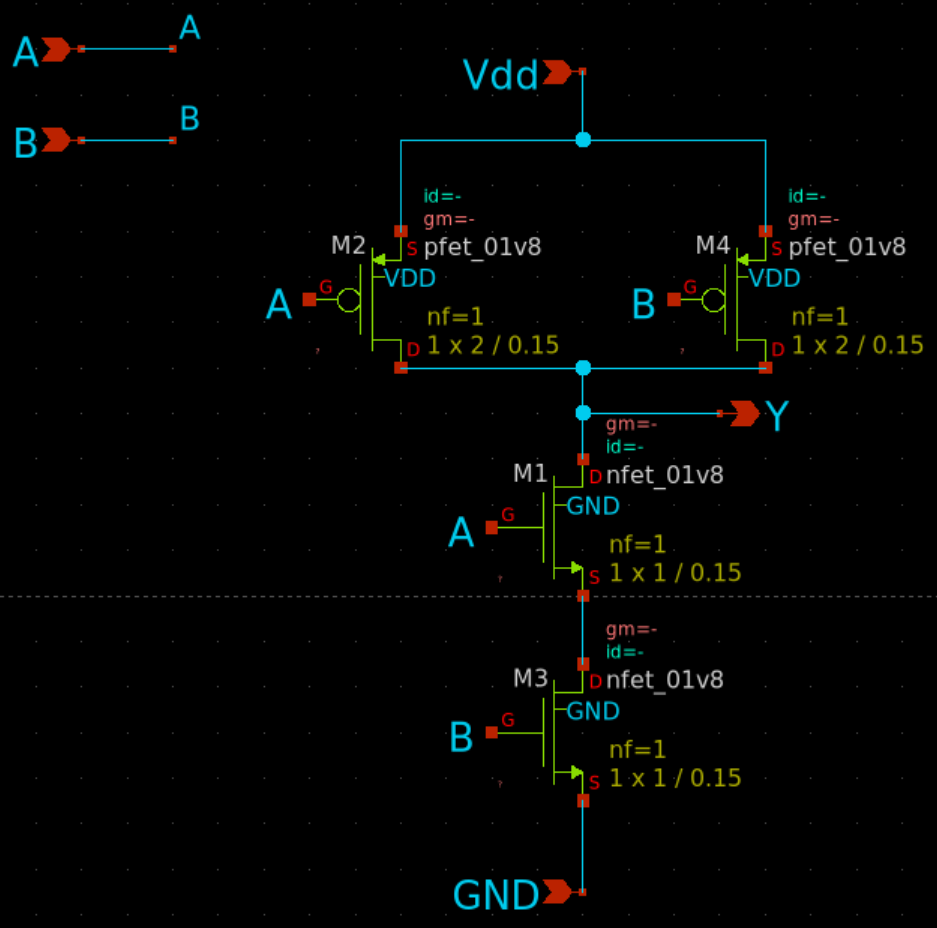
\includegraphics[width=0.4\textwidth]{nand_schematic.png}}
		\caption{NAND Circuit Schematic}
		\label{fig::nand_schematic}
	\end{figure}

	\noindent We also create a circuit symbol for the NAND gate, to allow reuse in other schematics. This circuit symbol is shown in Figure \ref{fig::nand_symbol}.
	
	\begin{figure}[H]
		\centerline{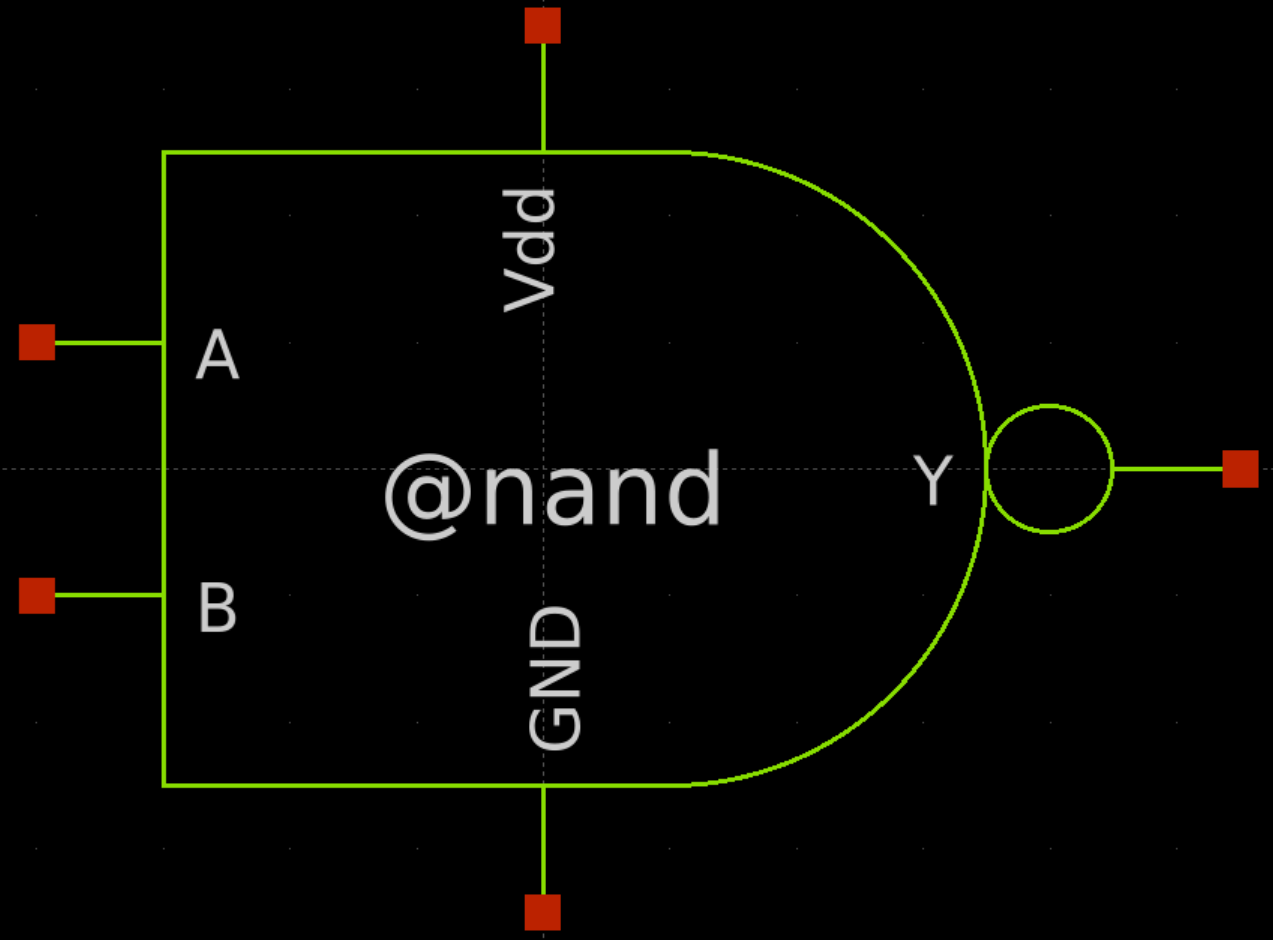
\includegraphics[width=0.4\textwidth]{nand_symbol.png}}
		\caption{NAND Circuit Symbol}
		\label{fig::nand_symbol}
	\end{figure}
	
	\subsubsection{Voltage Transfer Characteristics}
	
	In this section, we analyze the voltage transfer characteristics (VTC) of our NAND gate. For this analysis, we need to analyze the VTC for all combinations of inputs that lead to a logic level change. To generate the VTC in ngspice, we only need to consider one set of transitions because we care about the steady state output voltages for each input voltage. As such, we analyze the input voltages that result in high-to-low transitions. These voltages are dictated in Table \ref{table::nand_gate_high_to_low_transitions}.
	
	\begin{table}[H]
	\begin{center}
	\caption{Inputs that Create High to Low Transition for NAND Gate}
	\label{table::nand_gate_high_to_low_transitions}
	\begin{tabular}{| c | c |}
		\hline
		\texttt{a} & \texttt{b} \\
		\hline	
		$0 \rightarrow 1$ & $1$\\
		\hline	
		$1$ & $0 \rightarrow 1$\\
		\hline	
		$0 \rightarrow 1$ & $0 \rightarrow 1$\\
		\hline
	\end{tabular}
	\end{center}
	\end{table}
	
	\noindent The test circuit we use to generate the VTC for the first entry in the above table is shown in Figure \ref{fig::nand_vtc_test_sweep_va}.
	
	\begin{figure}[H]
		\centerline{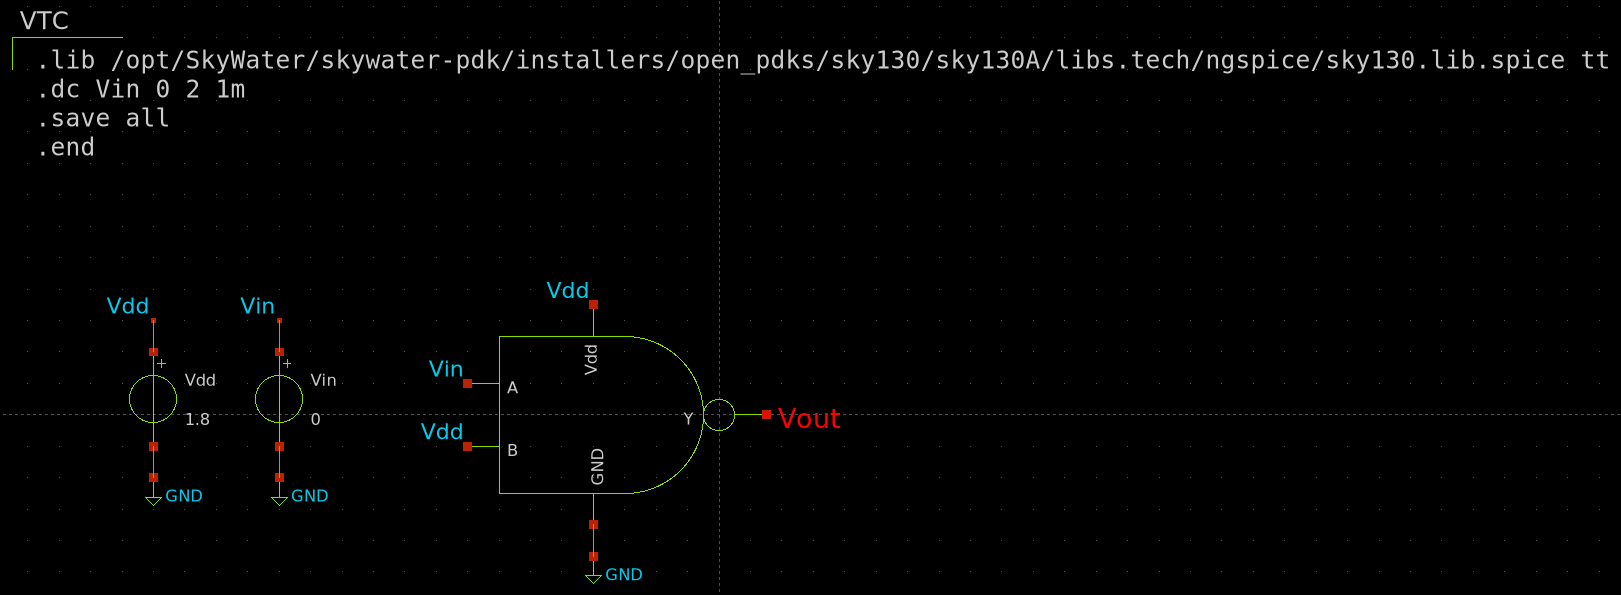
\includegraphics[width=0.8\textwidth]{nand_vtc_test_sweep_va.png}}
		\caption{NAND VTC Test Circuit for Variations of \texttt{a} with \texttt{b=1}}
		\label{fig::nand_vtc_test_sweep_va}
	\end{figure}	
	
	\noindent Using this test circuit, we perform DC analysis to generate the VTC and find \texttt{Vm}, which is the voltage at which \texttt{Vin = Vout}. The results of this analysis are shown in Figure \ref{fig::nand_vtc_sweep_va}.
	
	\begin{figure}[H]
		\centerline{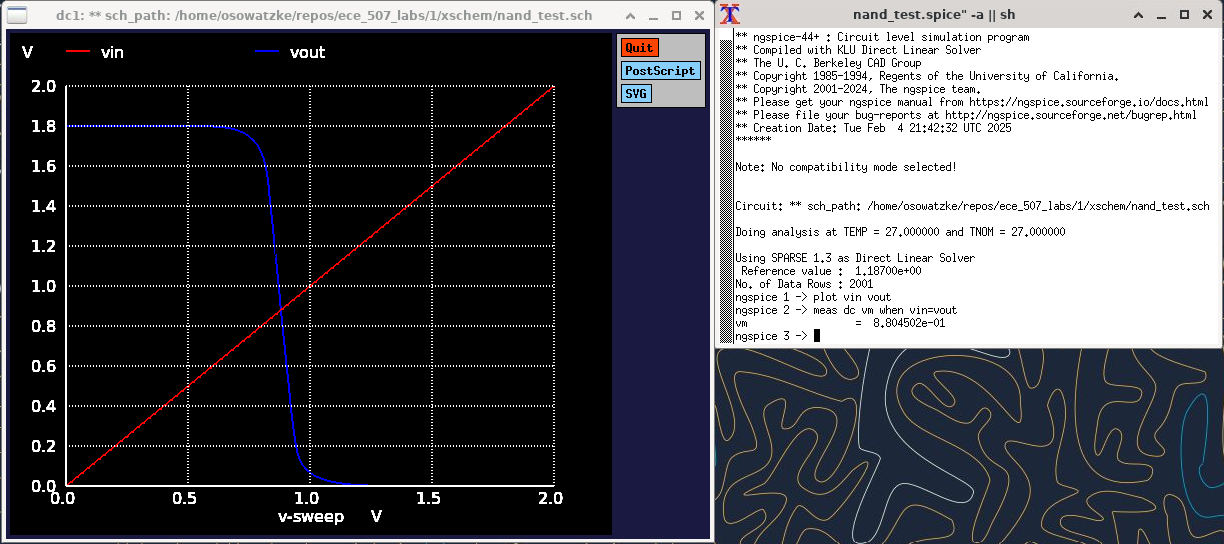
\includegraphics[width=0.8\textwidth]{nand_vtc_sweep_va.png}}
		\caption{NAND VTC Results for Variations of \texttt{a} with \texttt{b=1}}
		\label{fig::nand_vtc_sweep_va}
	\end{figure}
	
	Examining the results, we find that \texttt{Vm = 0.8257V}. With slight modifications to our test circuit, we perform similar analysis to find \texttt{Vm} for the other sets inputs listed in Table \ref{table::nand_gate_high_to_low_transitions}. These results are included in Table \ref{table::nand_gate_vm}.
	
	\begin{table}[H]
	\begin{center}
	\caption{\texttt{Vm} for Each Set of Inputs That Result in an Output Logic Level Change}
	\label{table::nand_gate_vm}
	\begin{tabular}{| c | c | c |}
		\hline
		\texttt{a} & \texttt{b} & \texttt{Vm}\\
		\hline	
		$0 \rightarrow 1$ & $1$ & $0.8257 \text{V}$\\
		\hline	
		$1$ & $0 \rightarrow 1$ & $0.8195 \text{V}$\\
		\hline	
		$0 \rightarrow 1$ & $0 \rightarrow 1$ & $0.9108 \text{V}$\\
		\hline
	\end{tabular}
	\end{center}
	\end{table}
	
	\noindent Reviewing our captured results, we see that \texttt{Vm} is dependent on the gate inputs. \texttt{Vm} is the largest when both gates switch at the same time. This makes sense because our pull-up network is strongest in this case, causing \texttt{Vm} to shift to the right.
	
	We can solve the IV equations to find \texttt{Vm} analytically. However, that can get complicated, especially for gates more complex than an inverter. When both inputs switch at the same time, we can instead use an equivalent inverter model described in \cite{cmos_vlsi_design, equivalent_inverter, inverter_dc_analysis}. In the equivalent inverter model, we treat the gate as an inverter and scale the NMOS and PMOS transistors to reflect the series and parallel transistors. For parallel connections, the equivalent resistance will be halved, and for series connections, the equivalent resistance will be doubled. For an NAND gate, this is equivalent to doubling the PMOS width (halving PMOS resistance) and halving NMOS width (doubling NMOS resistance).
	
	In an inverter, we can solve for \texttt{Vm} as follows:
	
	\begin{equation}
		\label{eq::vm}
		V_{M} = \frac{\left(V_{T_n} + \frac{V_{DSAT_n}}{2}\right) + r\left(V_{DD} + V_{T_p} + \frac{V_{DSAT_p}}{2}\right)}{1 + r}
	\end{equation}
	
	\noindent where:
	
	\begin{equation}
		\label{eq::beta_ratio}
		r = \frac{\beta_pV_{DSAT_p}}{\beta_nV_{DSAT_n}} = \frac{k_pW_pV_{DSAT_p}}{k_nW_nV_{DSAT_n}}
	\end{equation}
	
	\noindent In Equation \ref{eq::beta_ratio}, we use the widths of the transistors in the equivalent inverter. Then, we can substitute parameters from Appendix \ref{appendix::nmos_iv_characteristics} and \ref{appendix::pmos_iv_characteristics}, to find $Vm$. Doing so, we find that $V_m \approx 0.8404\ \text{V}$. Note that this estimate is off for a few reasons. First, Equation \ref{eq::vm} assumes that both devices are operating in the velocity saturation state which is not the case here ($|Vgs - Vt| < |V_{DSAT}|$ for both the NMOS and PMOS transistors). Secondly, the first order model presented in class do not do a good job of representing the current in the transition between linear and saturation regions, where $V_m$ unfortunately lies. 
	
	\subsubsection{Noise Analysis}
	\label{section::nand_noise_analysis}
	
	Using the test circuit shown in Figure \ref{fig::nand_vtc_test_sweep_va}, we can also measure the noise margins, which are defined follows:
	
	\begin{equation}
		NM_H = V_{OH} - V_{IH}
		\label{eq::noise_margin_high}
	\end{equation}
	
	\begin{equation}
		NM_L = V_{IL} - V_{OL}
		\label{eq::noise_margin_low}
	\end{equation}
	
	In the above formulas, $V_{IH}$ and $V_{IL}$ are defined as the unity points of the gain function, where the gain is defined as the derivative of the VTC. For the case in which we vary \texttt{a} with \texttt{b=1}, we can identify the unity gain points and solve for the noise margins.
	
	\begin{figure}[H]
		\centerline{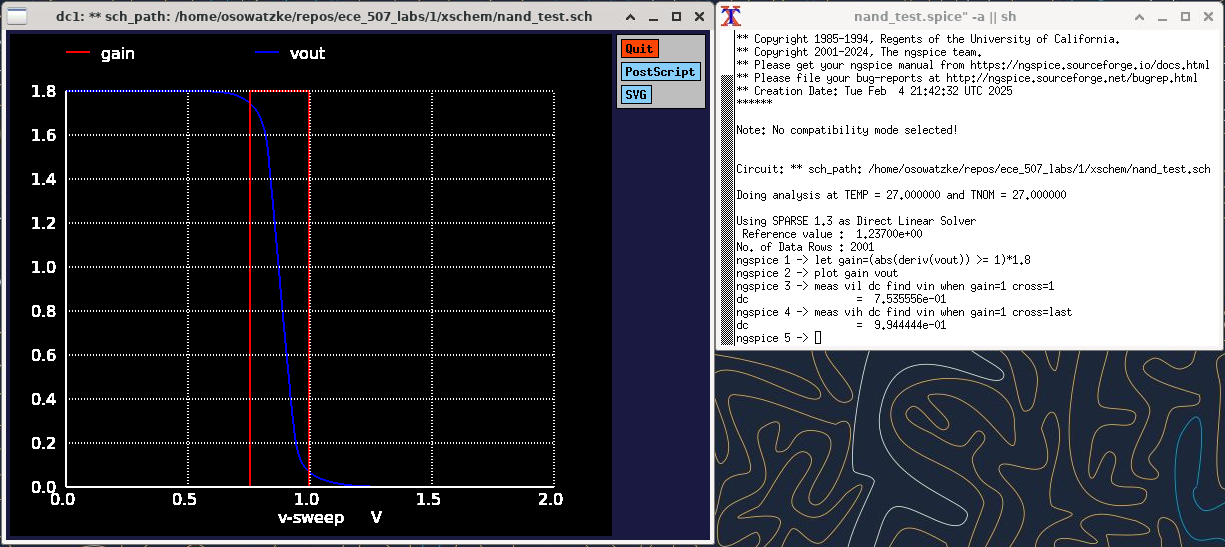
\includegraphics[width=0.8\textwidth]{nand_noise_analysis_sweep_va.png}}
		\caption{Measuring Noise Margins for the NAND Gate when \texttt{a} is Varied and \texttt{b=1}}	\label{fig::nand_noise_analysis_sweep_va}
	\end{figure}
	
	Examining the outputs shown in Figure \ref{fig::nand_noise_analysis_sweep_va}, we find that \texttt{Vil = 0.6926 V} and \texttt{Vih = 0.9264 V}. This implies that \texttt{Nmh = 1.8 V - 0.9264 V = 0.8736 V} and \texttt{Nml = 0.6926 V - 0 V = 0.6926 V}. With slight modifications to the test circuit, we can measure the noise margins for the sets of inputs listed in Table \ref{table::nand_gate_high_to_low_transitions}. Our results for this analysis are listed in Table \ref{table::nand_gate_noise_analysis}.
	
	\begin{table}[H]
	\begin{center}
	\caption{Noise Margins for Each Set of Inputs That Result in an Output Logic Level Change}
	\label{table::nand_gate_noise_analysis}
	\begin{tabular}{| c | c | c | c | c | c |}
		\hline
		\texttt{a} & \texttt{b} & \texttt{Vih} & \texttt{Vil} & \texttt{Nmh} & \texttt{Nml} \\
		\hline	
		$0 \rightarrow 1$ & $1$ & $0.9264 \text{V}$ & $0.6926 \text{V}$ & $0.8736 \text{V}$ & $0.6926 \text{V}$\\
		\hline	
		$1$ & $0 \rightarrow 1$ & $0.9184 \text{V}$ & $0.7116 \text{V}$ & $0.8816 \text{V}$ & $0.7116 \text{V}$\\
		\hline	
		$0 \rightarrow 1$ & $0 \rightarrow 1$ & $1.0224 \text{V}$ & $0.8046 \text{V}$ & $0.7776 \text{V}$ & $0.7776 \text{V}$\\
		\hline
	\end{tabular}
	\end{center}
	\end{table}
	
	We can also compute the noise margins using the equations presented in class. For this analysis, we consider the case where \texttt{a} and \texttt{b} vary together. This allows us to analyze the circuit with an equivalent inverter model. For our theoretical analysis, we also consider Figure \ref{fig::noise_margins_theory}, which is provided in \cite{rabaey_2003_digital}.
	
	\begin{figure}[H]
		\centerline{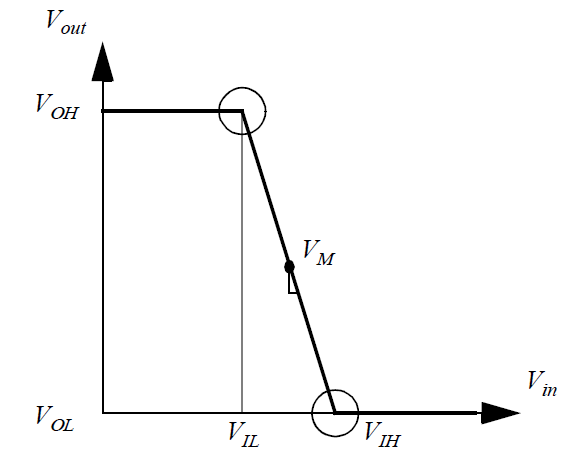
\includegraphics[width=0.4\textwidth]{noise_margins_theory.png}}
		\caption{Theoretical Noise Margins Analysis}
		\label{fig::noise_margins_theory}
	\end{figure}
	
	\noindent From the graph, we see that we can define $V_{IL}$ and $V_{IH}$ as follows:
	
	\begin{equation}
		V_{IH} = V_{M} - \frac{V_M}{g}
	\end{equation}
	
	\begin{equation}
		V_{IL} = V_{M} + \frac{V_{DD} - V_M}{g}
	\end{equation}
	
	\noindent For an inverter we can also define $g$ as follows:
	
	\begin{equation}
		g = -\frac{1}{I_D(V_M)}\frac{k_nV_{DSAT_n} + k_pV_{DSAT_p}}{\lambda_n - \lambda_p} \approx \frac{1 + r}{(V_M - V_{T_n} - V_{DSAT_n}/2)(\lambda_n - \lambda_p)}
	\end{equation}
	
	\noindent Substituting values from Appendix \ref{appendix::nmos_iv_characteristics} and \ref{appendix::pmos_iv_characteristics}, we find that $g \approx -265$. If we then use our theoretical estimate of $V_{M}$, we find that $V_{IL} \approx 0.8368\ \text{V}$ and $V_{IH} \approx 0.8436\ \text{V}$, which implies that $NM_L = 0.8368\ \text{V}$ and $NM_H \approx 0.9564\ \text{V}$. Note that this is  significantly different than our measured values. As discussed above, this is because $V_m$ is not in the velocity saturation region and because the level 1 model does not fit the transition between linear and saturation regions well.
	
	For our theoretical work, we can also use parameters measured in ngspice. We specifically use $Vm = 0.9108 V$ and $g = -14.83$, which we found in accordance with the steps in Figure \ref{fig::nand_noise_analysis_g_sweep_va_vb}.
	
	\begin{figure}[H]
		\centerline{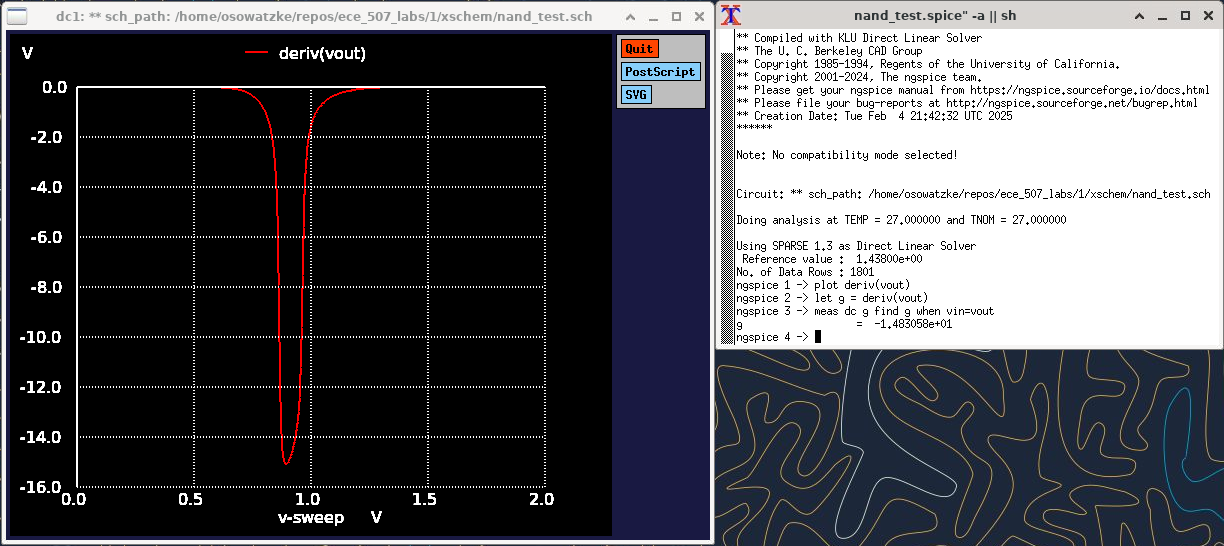
\includegraphics[width=0.8\textwidth]{nand_noise_analysis_g_sweep_va_vb.png}}
		\caption{Gain Measurement}
		\label{fig::nand_noise_analysis_g_sweep_va_vb}
	\end{figure}
	
	\noindent With the updated values, we find that $V_{IL} \approx 0.8508\ \text{V}$ and $V_{IH} \approx 0.9722\ \text{V}$, which implies that $NM_L = 0.8508\ \text{V}$ and $NM_H \approx 0.8278\ \text{V}$. These values are a lot closer to the theoretical values, but still contain a large margin of error.
	
	\subsubsection{Delay Analysis}
	
	In this section, we analyze the propagation delay of the NAND gate. To do so, we need to measure both the high-to-low propagation delay (\texttt{tphl}) and the low-to-high propagation delay. We measure \texttt{tphl} for each of the transitions listed in Table \ref{table::nand_gate_high_to_low_transitions}, and we measure \texttt{tplh} for each of the transitions listed in Table \ref{table::nand_gate_low_to_high_transitions}.
	
	\begin{table}[H]
	\begin{center}
	\caption{Inputs that Create Low-to-High Transition for NAND Gate}
	\label{table::nand_gate_low_to_high_transitions}
	\begin{tabular}{| c | c |}
		\hline
		\texttt{a} & \texttt{b} \\
		\hline	
		$1 \rightarrow 0$ & $1$\\
		\hline	
		$1$ & $1 \rightarrow 0$\\
		\hline	
		$1 \rightarrow 0$ & $1 \rightarrow 0$\\
		\hline
	\end{tabular}
	\end{center}
	\end{table}
	
	\noindent For variations of \texttt{a} with \texttt{b=1}, we can use the test circuit shown in Figure \ref{fig::nand_delay_test_sweep_va} to measure propagation delays. Note the input waveforms contains both rising an falling edges, so we can use it to measure \texttt{tphl} and \texttt{tplh}.

	\begin{figure}[H]
		\centerline{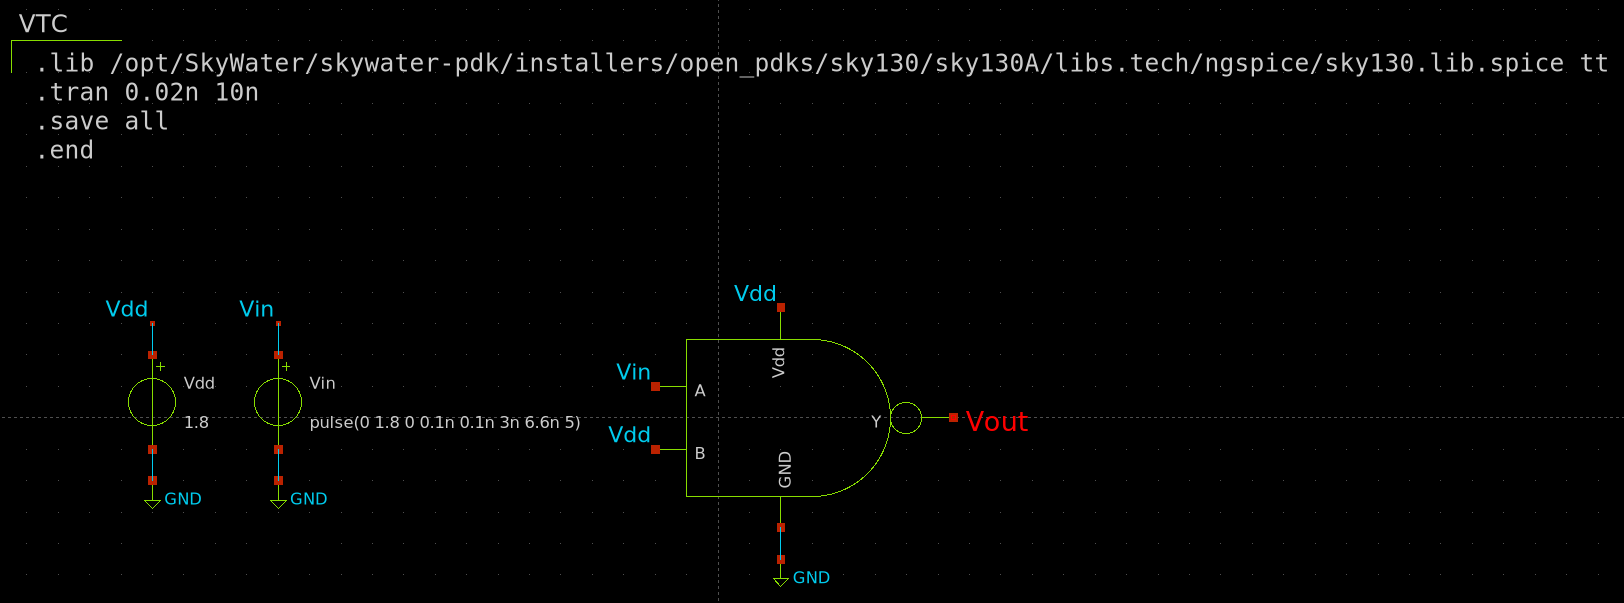
\includegraphics[width=0.8\textwidth]{nand_delay_test_sweep_va.png}}
		\caption{Test Circuit to Measure the Delay of the NAND Gate when \texttt{a} is Varied and \texttt{b=1}}
		\label{fig::nand_delay_test_sweep_va}
	\end{figure}
	
	\noindent Using the test circuit, we measure can measure \texttt{tphl} and \texttt{tplh} as follows:
	
	\begin{figure}[H]
		\centerline{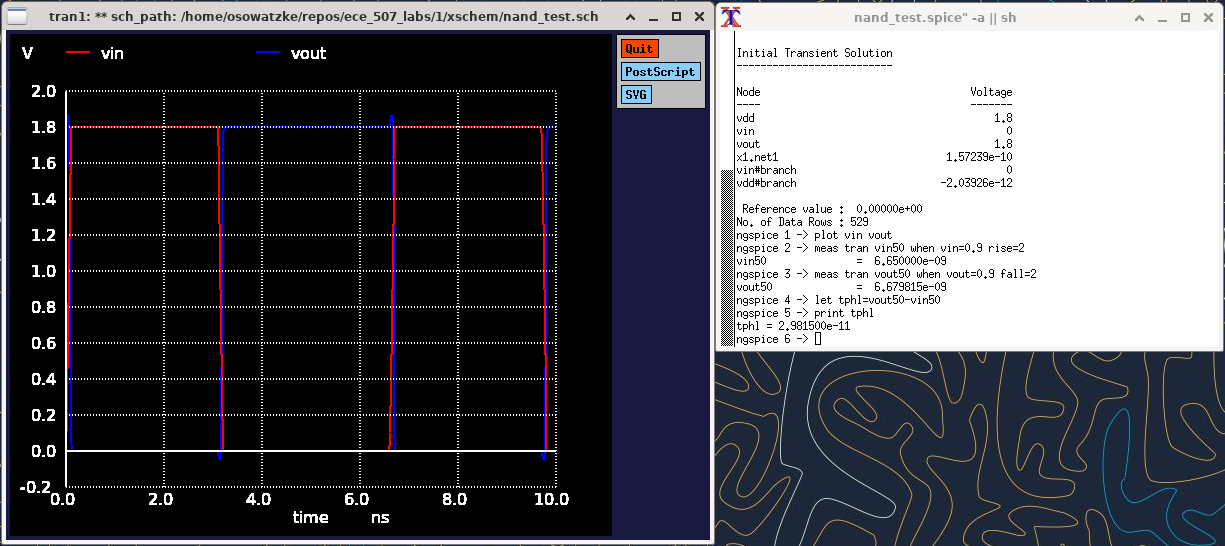
\includegraphics[width=0.8\textwidth]{nand_delay_sweep_va.png}}
		\caption{\texttt{tphl} Measurement for the NAND Gate when \texttt{a} is Varied and \texttt{b=1}}
		\label{fig::nand_delay_sweep_va}
	\end{figure}
	
	Examining the output results, we find that \texttt{tphl = 20.859 ps} for \texttt{a = }$0 \rightarrow 1$ and \texttt{b = 1}. Similarly, we find that \texttt{tphl = 33.178 ps} for \texttt{a = }$1 \rightarrow 0$ and \texttt{b = 1}. We perform similar analysis for the remaining transitions listed in Table \ref{table::nand_gate_high_to_low_transitions} and Table \ref{table::nand_gate_high_to_low_transitions}. Our results are summarized in Table \ref{table::nand_gate_delay_analysis}.
	
	\begin{table}[H]
	\begin{center}
	\caption{Propagation Delays for Each Transition That Result in an Output Logic Level Change}
	\label{table::nand_gate_delay_analysis}
	\begin{tabular}{| c | c | c || c | c | c |}
		\hline
		\texttt{a} & \texttt{b} & \texttt{tphl} & \texttt{a} & \texttt{b} & \texttt{tplh} \\
		\hline	
		$0 \rightarrow 1$ & $1$ & $20.859\ \text{ps}$ & $1 \rightarrow 0$ & $1$ & $33.178\ \text{ps}$\\
		\hline	
		$1$ & $0 \rightarrow 1$ & $28.146\ \text{ps}$ & $1$ & $1 \rightarrow 0$ & $48.137\ \text{ps}$\\
		\hline	
		$0 \rightarrow 1$ & $0 \rightarrow 1$ & $29.297\ \text{ps}$ & $1 \rightarrow 0$ & $1 \rightarrow 0$ & $26.097\ \text{ps}$\\
		\hline
	\end{tabular}
	\end{center}
	\end{table}
	
	\subsubsection{Power Analysis}
	
	In this section, we analyze the power consumption of our NAND gate. Similar to what we did above, we analyze the power consumption for each input variation that results in an output logical level change. For our input, we used a pulsed source. This allows us to capture both rising and falling edges of the output. We use the test circuit shown in Figure \ref{fig::nand_power_test_sweep_va} to measure the power consumption for variations of \texttt{a} with \texttt{b=1}. For this analysis, we have also attached a parasitic capacitance to the gate output.
	
	\begin{figure}[H]
		\centerline{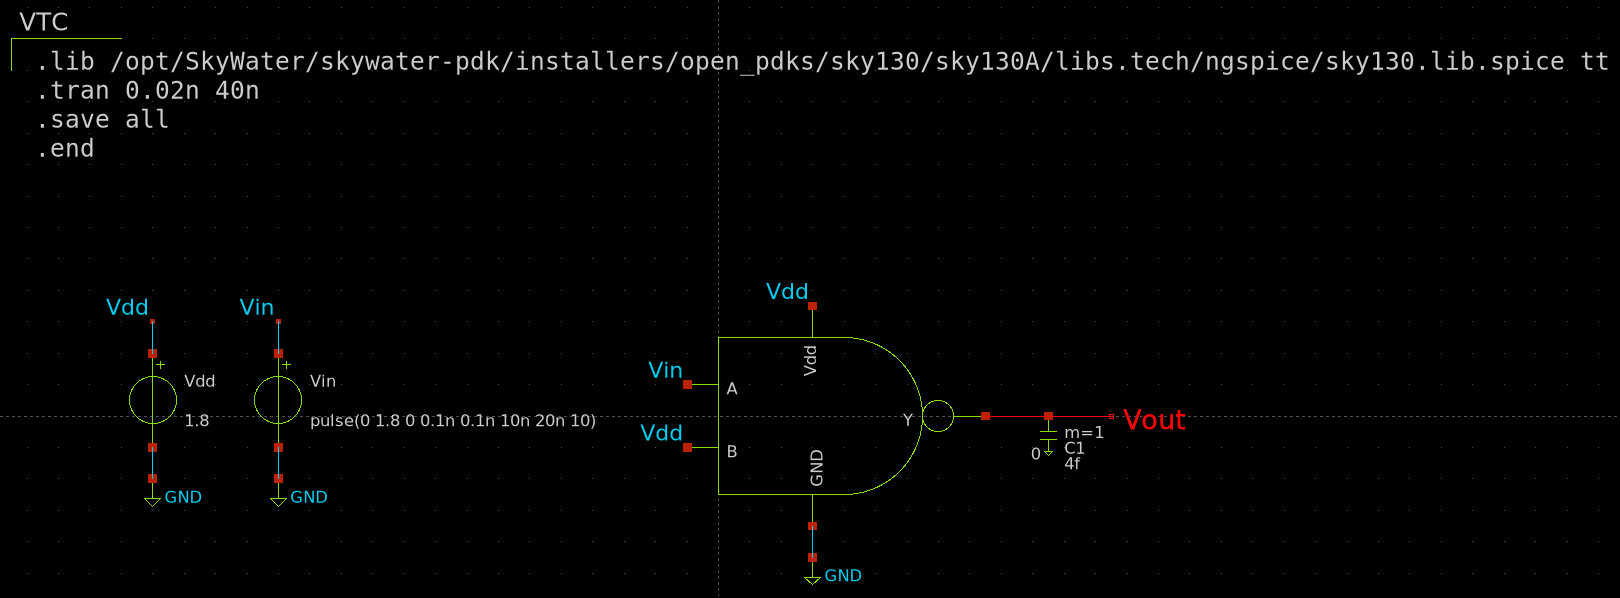
\includegraphics[width=0.8\textwidth]{nand_power_test_sweep_va.png}}
		\caption{Test Circuit to Measure the Power Consumption of the NAND Gate when \texttt{a} is Varied and \texttt{b=1}}
		\label{fig::nand_power_test_sweep_va}
	\end{figure}
	
	\noindent Using the test circuit, we measure the power consumption as follows:
	
	\begin{figure}[H]
		\centerline{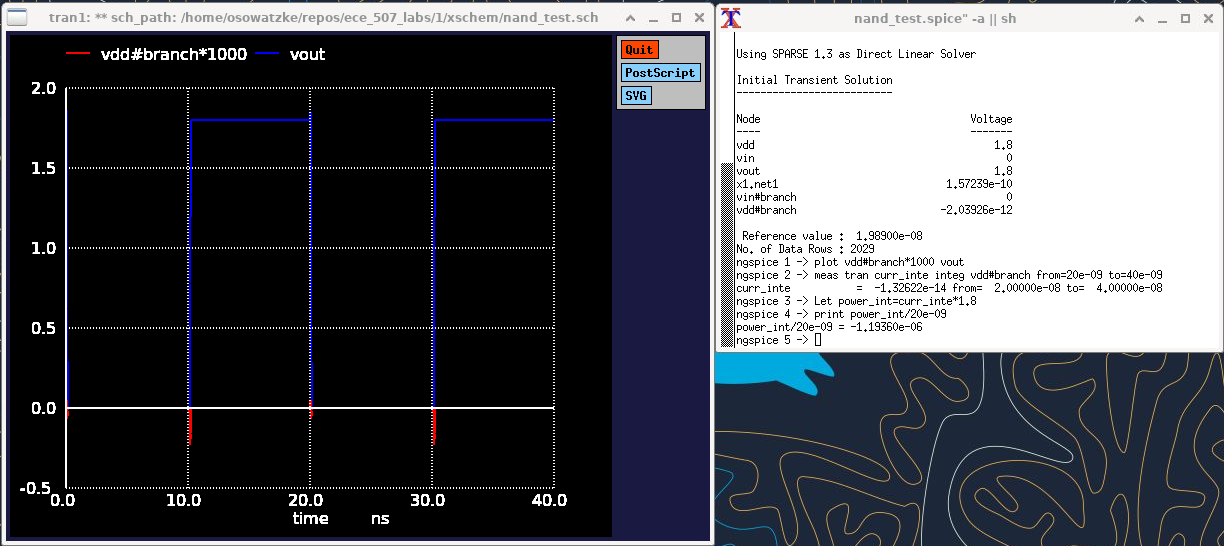
\includegraphics[width=0.8\textwidth]{nand_power_sweep_va.png}}
		\caption{Power Consumption of the NAND Gate when \texttt{a} is Varied and \texttt{b=1}}
		\label{fig::nand_power_sweep_va}
	\end{figure}
	
	\noindent Examining the results, we find that the power consumption is $1.34880{\mu}W$. Note that this power estimate includes the effects of the rising and falling edges of \texttt{a}. We can perform similar analysis for other variations of the input. Our results for this work are summarized in Table \ref{table::nand_gate_power_analysis}.
	
	\begin{table}[H]
	\begin{center}
	\caption{NAND Gate Power Consumption for Different Input Variations}
	\label{table::nand_gate_power_analysis}
	\begin{tabular}{| c | c | c |}
		\hline
		\texttt{a} & \texttt{b} & \texttt{Power}\\
		\hline	
		$0 \rightarrow 1 \rightarrow 0$ & $1$ & $1.34880{\mu}W$ \\
		\hline	
		$1$ & $0 \rightarrow 1 \rightarrow 0$ & $1.88943{\mu}W$ \\
		\hline	
		$0 \rightarrow 1 \rightarrow 0$ & $0 \rightarrow 1 \rightarrow 0$ & $1.44446{\mu}W$\\
		\hline
	\end{tabular}
	\end{center}
	\end{table}
	
	\subsection{NOR Gate}
	
	\subsubsection{Design}
	
	The NOR gate pull-down circuit is composed of two parallel NMOS transistors. The pull-up circuit is the complement of the pull-down circuit and is composed of two PMOS transistors in series. For analysis, we can create an equivalent inverter from the NOR gate. In this equivalent inverter, the channel length of the PMOS transistor is doubled because the PMOS transistors in the NOR gate are laid out in series. (This is equivalent to halving the width of the transistor). The NOR gate pull-down circuit is on when either transistor is on. However, for analysis, we consider the worst (slowest) case, when only one transistor is on. Therefore, the NMOS transistor width in the equivalent inverter remains unchanged.
	
	For an inverter, we know that we need to make the width of the PMOS transistor twice as large as the width NMOS transistor because the mobility of holes is lower than the mobility of electrons. We can map these sizes back to the NOR gate. Doing so, we find that NMOS transistor width in the NOR gate should be the same as the inverter, and the PMOS transistor width should be doubled. To match the behavior of the inverter with a NMOS width of 1 and a PMOS width of 2, we should make the NMOS width 1 and the PMOS width 4. The NOR gate circuit with these transistor widths is shown in Figure \ref{fig::nor_schematic}.
	
	\begin{figure}[H]
		\centerline{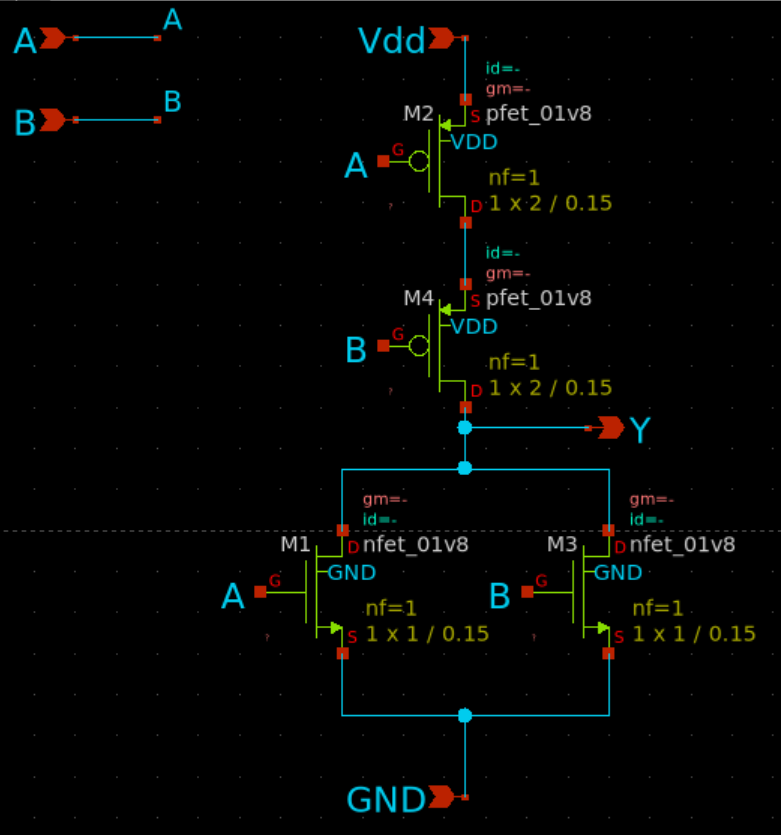
\includegraphics[width=0.4\textwidth]{nor_schematic.png}}
		\caption{NOR Circuit Schematic}
		\label{fig::nor_schematic}
	\end{figure}
	
	\noindent We also create a circuit symbol for the NOR gate, to allow reuse in other schematics. This circuit symbol is shown in Figure \ref{fig::nor_symbol}.
	
	\begin{figure}[H]
		\centerline{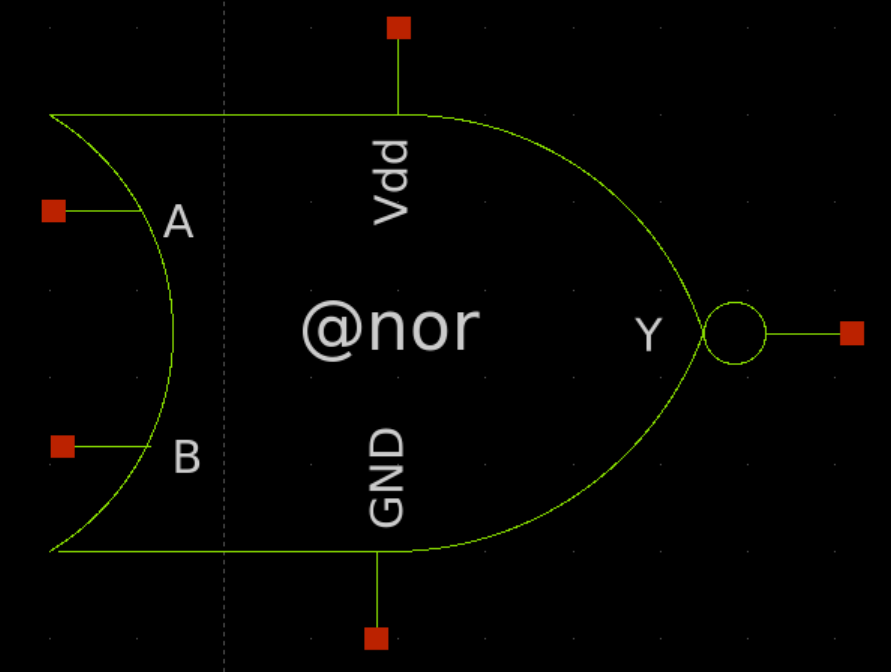
\includegraphics[width=0.4\textwidth]{nor_symbol.png}}
		\caption{NOR Circuit Symbol}
		\label{fig::nor_symbol}
	\end{figure}

	\subsubsection{Voltage Transfer Characteristics}
	
	In this section, we analyze the voltage transfer characteristics (VTC) of our NOR gate. For this analysis, we need to analyze the VTC for all combinations of inputs that lead to a logic level change. To generate the VTC in ngspice, we only need to consider one set of transitions because we care about the steady state output voltages for each input voltage. As such, we analyze the input voltages that result in high-to-low transitions. These voltages are dictated in Table \ref{table::nor_gate_high_to_low_transitions}.
	
	\begin{table}[H]
	\begin{center}
	\caption{Inputs that Create High to Low Transition for NOR Gate}
	\label{table::nor_gate_high_to_low_transitions}
	\begin{tabular}{| c | c |}
		\hline
		\texttt{a} & \texttt{b} \\
		\hline	
		$0 \rightarrow 1$ & $0$\\
		\hline	
		$0$ & $0 \rightarrow 1$\\
		\hline	
		$0 \rightarrow 1$ & $0 \rightarrow 1$\\
		\hline
	\end{tabular}
	\end{center}
	\end{table}
	
	\noindent The test circuit we use to generate the VTC for the first entry in the above table is shown in Figure \ref{fig::nor_vtc_test_sweep_va}.
	
	\begin{figure}[H]
		\centerline{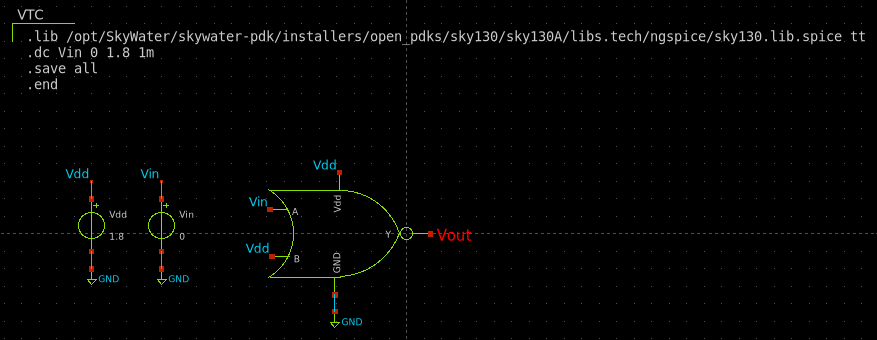
\includegraphics[width=0.8\textwidth]{nor_vtc_test_sweep_va.png}}
		\caption{NOR VTC Test Circuit for Variations of \texttt{a} with \texttt{b=0}}
		\label{fig::nor_vtc_test_sweep_va}
	\end{figure}	
	
	\noindent Using this test circuit, we perform DC analysis to generate the VTC and find \texttt{Vm}, which is the voltage at which \texttt{Vin = Vout}. The results of this analysis are shown in Figure \ref{fig::nor_vtc_sweep_va}.
	
	\begin{figure}[H]
		\centerline{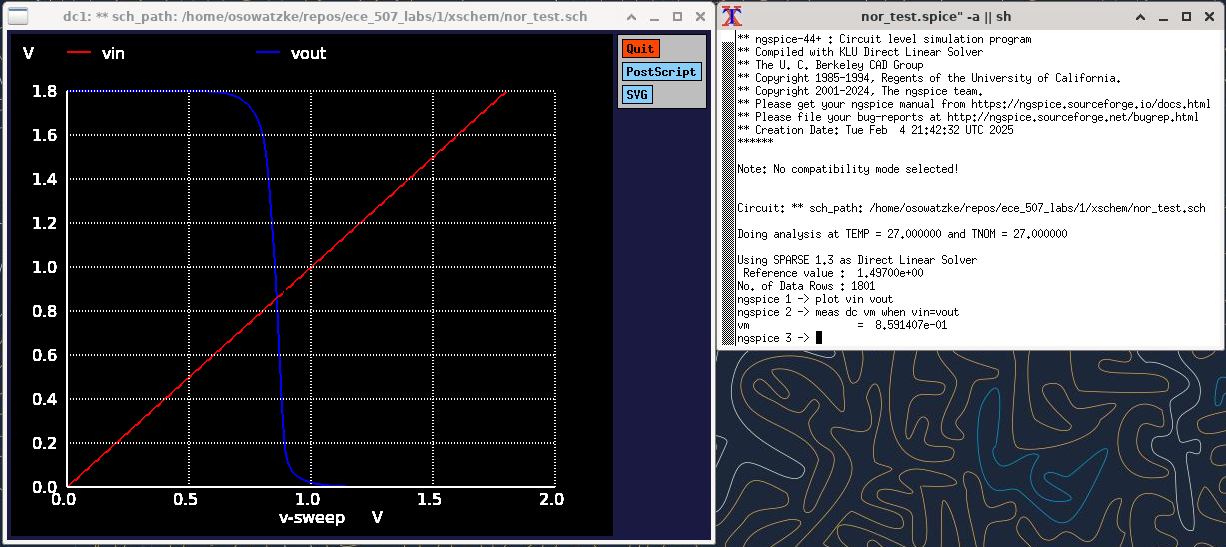
\includegraphics[width=0.8\textwidth]{nor_vtc_sweep_va.png}}
		\caption{NOR VTC Results for Variations of \texttt{a} with \texttt{b=0}}
		\label{fig::nor_vtc_sweep_va}
	\end{figure}
	
	Examining the results, we find that \texttt{Vm = 0.8952V}. With slight modifications to our test circuit, we perform similar analysis to find \texttt{Vm} for the other sets inputs listed in Table \ref{table::nor_gate_high_to_low_transitions}. These results are included in Table \ref{table::nor_gate_vm}.
	
	\begin{table}[H]
	\begin{center}
	\caption{\texttt{Vm} for Each Set of Inputs That Result in an Output Logic Level Change}
	\label{table::nor_gate_vm}
	\begin{tabular}{| c | c | c |}
		\hline
		\texttt{a} & \texttt{b} & \texttt{Vm}\\
		\hline	
		$0 \rightarrow 1$ & $0$ & $0.8952 \text{V}$\\
		\hline	
		$1$ & $0 \rightarrow 1$ & $0.8919 \text{V}$\\
		\hline	
		$0 \rightarrow 1$ & $0 \rightarrow 1$ & $0.8078 \text{V}$\\
		\hline
	\end{tabular}
	\end{center}
	\end{table}
	
	\noindent Reviewing our captured results, we see that \texttt{Vm} is dependent on the gate inputs. \texttt{Vm} is the smallest when both gates switch at the same time. This makes sense because our pull-down network is strongest in this case, causing \texttt{Vm} to shift to the left.
	
	\subsubsection{Noise Analysis}
	
	Using the test circuit shown in Figure \ref{fig::nor_vtc_test_sweep_va}, we can also measure the noise margins, which are defined by Equations \ref{eq::noise_margin_high} and \ref{eq::noise_margin_low}. In the referenced formulas, $V_{IH}$ and $V_{IL}$ are defined as the unity points of the gain function, where the gain is defined as the derivative of the VTC. For the case in which we vary \texttt{a} with \texttt{b=0}, we can identify the unity gain points and solve for the noise margins.
	
	\begin{figure}[H]
		\centerline{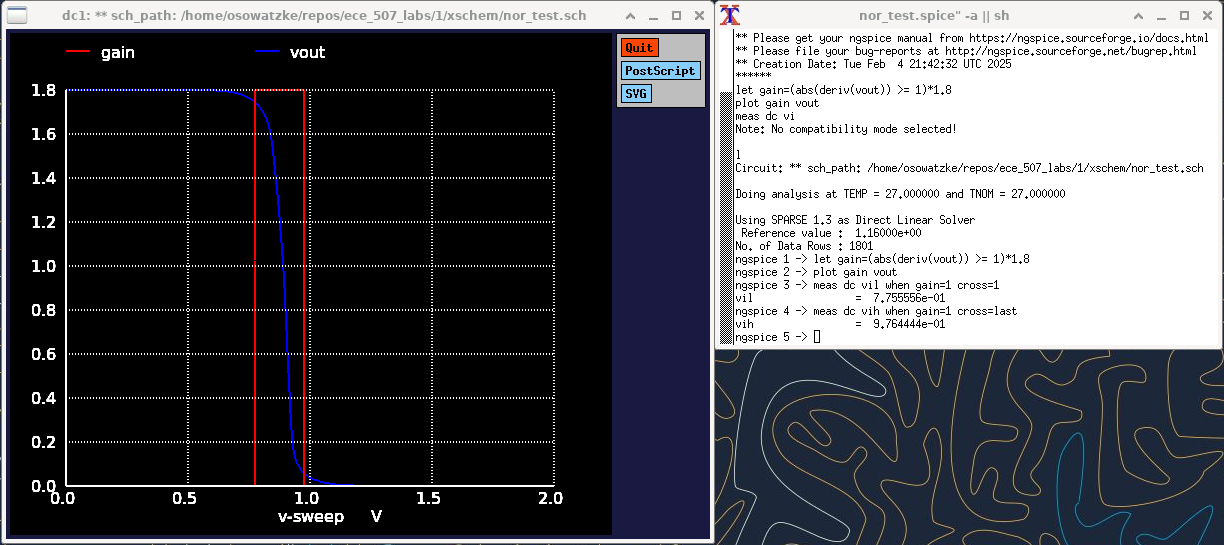
\includegraphics[width=0.8\textwidth]{nor_noise_analysis_sweep_va.png}}
		\caption{Measuring Noise Margins for the NOR Gate when \texttt{a} is Varied and \texttt{b=0}}	\label{fig::nor_noise_analysis_sweep_va}
	\end{figure}
	
	Examining the outputs shown in Figure \ref{fig::nor_noise_analysis_sweep_va}, we find that \texttt{Vil = 0.7756 V} and \texttt{Vih = 0.9764 V}. This implies that \texttt{Nmh = 1.8 V - 0.9764 V = 0.8326 V} and \texttt{Nml = 0.7756 V - 0 V = 0.7756 V}. With slight modifications to the test circuit, we can measure the noise margins for the sets of inputs listed in Table \ref{table::nor_gate_high_to_low_transitions}. Our results for this analysis are listed in Table \ref{table::nor_gate_noise_analysis}.
	
	\begin{table}[H]
	\begin{center}
	\caption{Noise Margins for Each Set of Inputs That Result in an Output Logic Level Change}
	\label{table::nor_gate_noise_analysis}
	\begin{tabular}{| c | c | c | c | c | c |}
		\hline
		\texttt{a} & \texttt{b} & \texttt{Vih} & \texttt{Vil} & \texttt{Nmh} & \texttt{Nml} \\
		\hline	
		$0 \rightarrow 1$ & $0$ & $0.9764 \text{V}$ & $0.7756 \text{V}$ & $0.8326 \text{V}$ & $0.7756 \text{V}$\\
		\hline	
		$1$ & $0 \rightarrow 1$ & $1.0134 \text{V}$ & $0.7706 \text{V}$ & $0.7660 \text{V}$ & $0.7706 \text{V}$\\
		\hline	
		$0 \rightarrow 1$ & $0 \rightarrow 1$ & $0.7006 \text{V}$ & $0.8844 \text{V}$ & $0.9156 \text{V}$ & $0.7006 \text{V}$\\
		\hline
	\end{tabular}
	\end{center}
	\end{table}
	
	\subsubsection{Delay Analysis}
	
	In this section, we analyze the propagation delay of the NOR gate. To do so, we need to measure both the high-to-low propagation delay (\texttt{tphl}) and the low-to-high propagation delay. We measure \texttt{tphl} for each of the transitions listed in Table \ref{table::nor_gate_high_to_low_transitions}, and we measure \texttt{tplh} for each of the transitions listed in Table \ref{table::nor_gate_low_to_high_transitions}.
	
	\begin{table}[H]
	\begin{center}
	\caption{Inputs that Create Low-to-High Transition for NOR Gate}
	\label{table::nor_gate_low_to_high_transitions}
	\begin{tabular}{| c | c |}
		\hline
		\texttt{a} & \texttt{b} \\
		\hline	
		$1 \rightarrow 0$ & $0$\\
		\hline	
		$0$ & $1 \rightarrow 0$\\
		\hline	
		$1 \rightarrow 0$ & $1 \rightarrow 0$\\
		\hline
	\end{tabular}
	\end{center}
	\end{table}
	
	\noindent For variations of \texttt{a} with \texttt{b=0}, we can use the test circuit shown in Figure \ref{fig::nor_delay_test_sweep_va} to measure propagation delays. Note the input waveforms contains both rising an falling edges, so we can use it to measure \texttt{tphl} and \texttt{tplh}.

	\begin{figure}[H]
		\centerline{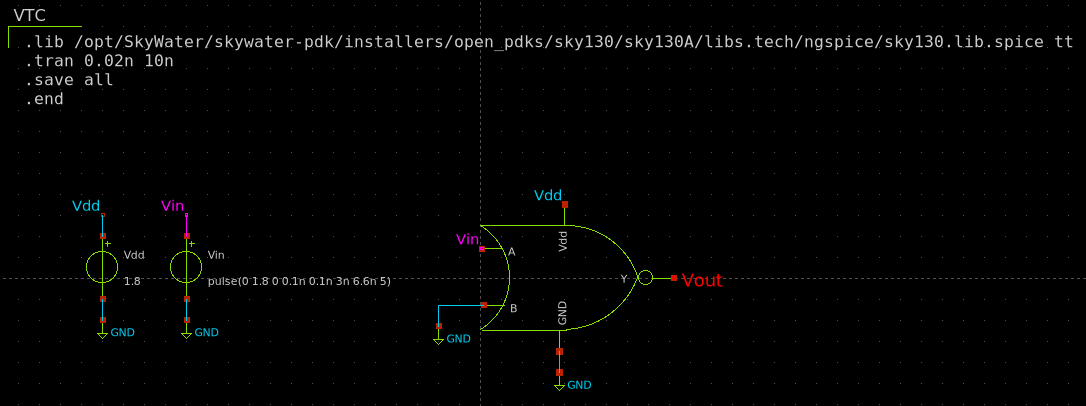
\includegraphics[width=0.8\textwidth]{nor_delay_test_sweep_va.png}}
		\caption{Test Circuit to Measure the Delay of the NOR Gate when \texttt{a} is Varied and \texttt{b=0}}
		\label{fig::nor_delay_test_sweep_va}
	\end{figure}
	
	\noindent Using the test circuit, we measure can measure \texttt{tphl} and \texttt{tplh} as follows:
	
	\begin{figure}[H]
		\centerline{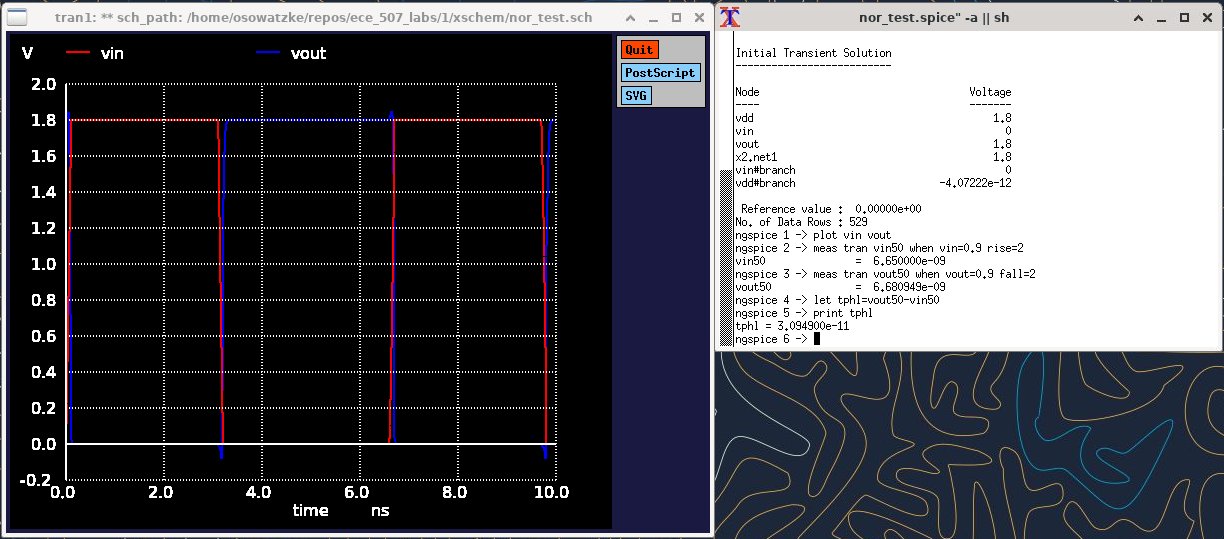
\includegraphics[width=0.8\textwidth]{nor_delay_sweep_va.png}}
		\caption{\texttt{tphl} Measurement for the NAND Gate when \texttt{a} is Varied and \texttt{b=0}}
		\label{fig::nor_delay_sweep_va}
	\end{figure}
	
	Examining the output results, we find that \texttt{tphl = 44.975 ps} for \texttt{a = }$0 \rightarrow 1$ and \texttt{b = 1}. Similarly, we find that \texttt{tphl = 45.841 ps} for \texttt{a = }$1 \rightarrow 0$ and \texttt{b = 0}. We perform similar analysis for the remaining transitions listed in Table \ref{table::nor_gate_high_to_low_transitions} and Table \ref{table::nor_gate_low_to_high_transitions}. Our results are summarized in Table \ref{table::nor_gate_delay_analysis}.
	
	\begin{table}[H]
	\begin{center}
	\caption{Propagation Delays for Each Transition That Result in an Output Logic Level Change}
	\label{table::nor_gate_delay_analysis}
	\begin{tabular}{| c | c | c || c | c | c |}
		\hline
		\texttt{a} & \texttt{b} & \texttt{tphl} & \texttt{a} & \texttt{b} & \texttt{tplh} \\
		\hline	
		$0 \rightarrow 1$ & $0$ & $44.975\ \text{ps}$ & $1 \rightarrow 0$ & $0$ & $45.841\ \text{ps}$\\
		\hline	
		$0$ & $0 \rightarrow 1$ & $29.139\ \text{ps}$ & $0$ & $1 \rightarrow 0$ & $29.942\ \text{ps}$\\
		\hline	
		$0 \rightarrow 1$ & $0 \rightarrow 1$ & $22.437\ \text{ps}$ & $1 \rightarrow 0$ & $1 \rightarrow 0$ & $40.997\ \text{ps}$\\
		\hline
	\end{tabular}
	\end{center}
	\end{table}
	
	\subsubsection{Power Analysis}
	
	In this section, we analyze the power consumption of our NOR gate. Similar to what we did above, we analyze the power consumption for each input variation that results in an output logical level change. For our input, we used a pulsed source. This allows us to capture both rising and falling edges of the output. We use the test circuit shown in Figure \ref{fig::nor_power_test_sweep_va} to measure the power consumption for variations of \texttt{a} with \texttt{b=0}. For this analysis, we have also attached a parasitic capacitance to the gate output.
	
	\begin{figure}[H]
		\centerline{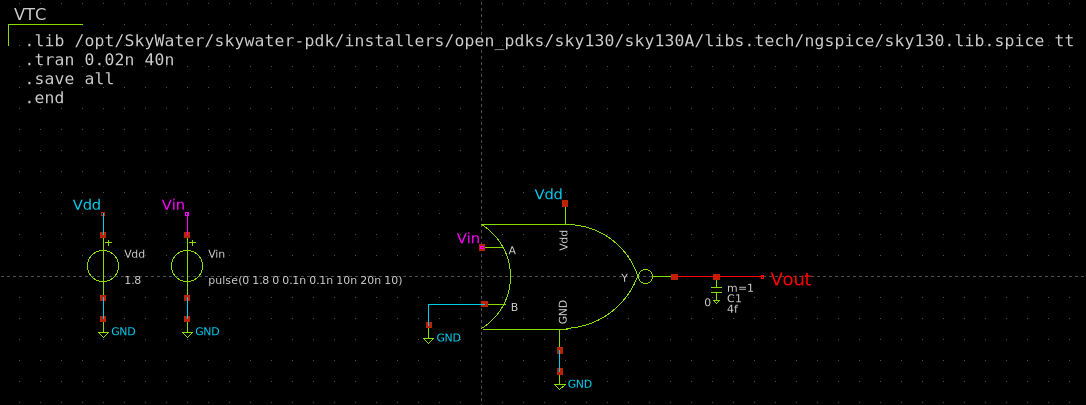
\includegraphics[width=0.8\textwidth]{nor_power_test_sweep_va.png}}
		\caption{Test Circuit to Measure the Power Consumption of the NOR Gate when \texttt{a} is Varied and \texttt{b=0}}
		\label{fig::nor_power_test_sweep_va}
	\end{figure}
	
	\noindent Using the test circuit, we measure the power consumption as follows:
	
	\begin{figure}[H]
		\centerline{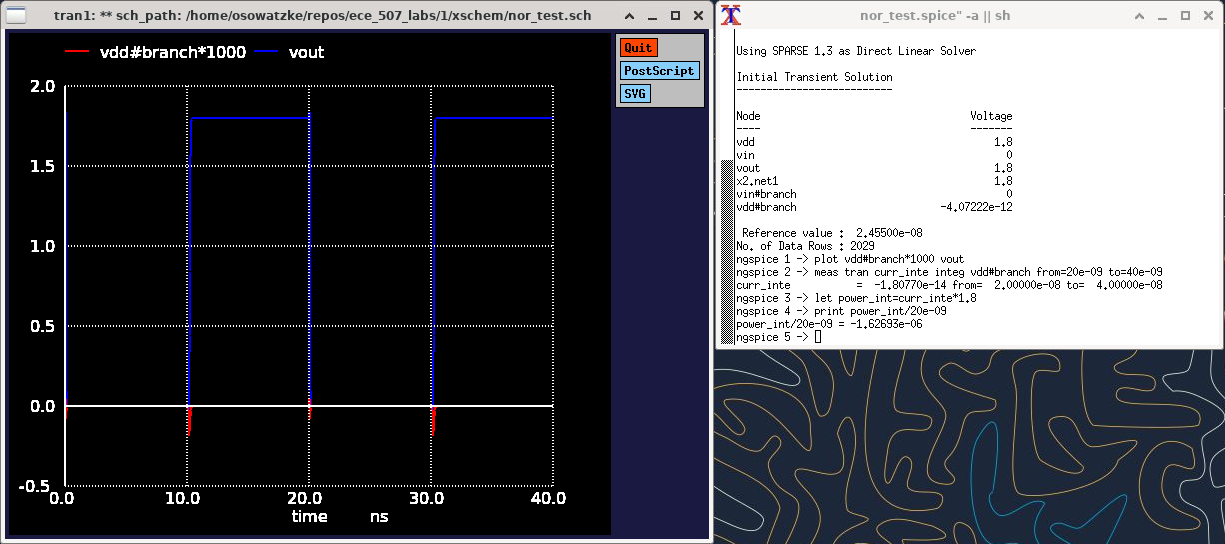
\includegraphics[width=0.8\textwidth]{nor_power_sweep_va.png}}
		\caption{Power Consumption of the NOR Gate when \texttt{a} is Varied and \texttt{b=0}}
		\label{fig::nor_power_sweep_va}
	\end{figure}
	
	\noindent Examining the results, we find that the power consumption is $2.28022{\mu}W$. Note that this power estimate includes the effects of the rising and falling edges of \texttt{a}. We can perform similar analysis for other variations of the input. Our results for this work are summarized in Table \ref{table::nor_gate_power_analysis}.
	
	\begin{table}[H]
	\begin{center}
	\caption{NOR Gate Power Consumption for Different Input Variations}
	\label{table::nor_gate_power_analysis}
	\begin{tabular}{| c | c | c |}
		\hline
		\texttt{a} & \texttt{b} & \texttt{Power}\\
		\hline	
		$0 \rightarrow 1 \rightarrow 0$ & $1$ & $2.28022{\mu}W$ \\
		\hline	
		$1$ & $0 \rightarrow 1 \rightarrow 0$ & $1.3767{\mu}W$ \\
		\hline	
		$0 \rightarrow 1 \rightarrow 0$ & $0 \rightarrow 1 \rightarrow 0$ & $1.61932{\mu}W$\\
		\hline
	\end{tabular}
	\end{center}
	\end{table}
	
	\subsection{NAND Gate}

	\begin{align}
		I_{ds_p} &= -k_p\frac{W_p}{L}V_{dsat_p}\left(V_{gs_p} - V_{T0_p} - \frac{V_{dsat_p}}{2}\right)\left(1 + {\lambda_p}V_{ds_p}\right) \\
		&= -k_p\frac{W}{L}V_{dsat_p}\left(V_m - V_{dd} - V_{T0_p} - \frac{V_{dsat_p}}{2}\right)\left(1 + {\lambda_p}(V_m - V_{dd})\right)
	\end{align}
	
	\begin{align}
		I_{ds_n} &= k_n\frac{W_n}{L}V_{dsat_n}\left(V_{gs_n} - V_{T0_n} - \frac{V_{dsat_n}}{2}\right)\left(1 + {\lambda_n}V_{ds_n}\right) \\
		&= k_n\frac{W_n}{L}V_{dsat_n}\left(V_m - V_{T0_n} - \frac{V_{dsat_n}}{2}\right)\left(1 + {\lambda_n}V_m\right)
	\end{align}
	
	Using KCL, we know that:
	
	\begin{equation}
		I_{ds_n} + I_{ds_p} = 0
	\end{equation}
	
	Solving numerically, using the parameters in Table \ref{table::nmos_params} we find that $V_m = 0.8422 V$.
	
	\begin{equation}
		V_{IH} = V_{M} - \frac{V_M}{g}
	\end{equation}
	
	\begin{equation}
		V_{IL} = V_{M} + \frac{V_{DD} - V_M}{g}
	\end{equation}
	
	\begin{equation}
		g = -\frac{1}{I_D(V_M)}\frac{k_nV_{DSAT_n} + k_pV_{DSAT_p}}{\lambda_n - \lambda_p} \approx \frac{1 + r}{(V_M - V_{T_n} - V_{DSAT_n}/2)(\lambda_n - \lambda_p)}
	\end{equation}
	
	\begin{equation}
		t_p = 0.69R_{on}C_L
	\end{equation}
	
	\begin{equation}
		P_{switching} = {\alpha}CV_{DD}^2f
	\end{equation}
	
	\bibliographystyle{IEEEtran}
	\bibliography{IEEEabrv,sources}
	\pagebreak
	\appendix
	\section{NMOS IV Characteristics}
	\label{appendix::nmos_iv_characteristics}
	
	In this appendix, we fit a first-order mosfet model to NMOS IV characteristics measured with the sky130A PDK. This enables us to use the equations presented in class to perform first-order analysis of our CMOS gate. We start by estimating the threshold voltage of the NMOS transistor. To perform this measurement, we use the linear extrapolation (or maximum gm) method given in \cite{cmos_vlsi_design}. Our ngspice flowchart for this analysis is given in Figure \ref{fig::nmos_vt_meas_schem}.
	
	\begin{figure}[H]
		\centerline{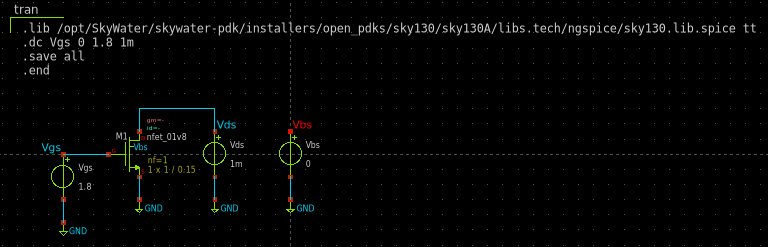
\includegraphics[width=0.8\textwidth]{nmos_vt_meas_schem.png}}
		\caption{NGSPICE Schematic Used to Measure the NMOS Threshold Voltage}
		\label{fig::nmos_vt_meas_schem}
	\end{figure}
	
	\noindent Using the flowchart, we examine the drain current for the NMOS transistor in the linear region of operation. In this region, the drain current of the NMOS transistor is given as follows:
	
	\begin{equation}
		I_{ds} = k_n\frac{W_n}{L}\left(V_{gs} - V_{t_n} - \frac{V_{ds}}{2}\right)V_{ds}
	\end{equation}
	
	\noindent To fit the IV characteristics, we estimate the $I_{ds}$ curve with a line that is tangent to the point with maximum-slope. We then define $V_t$ as the voltage at which the estimated current is zero. This procedure is illustrated in Figure \ref{fig::nmos_vt_meas}, which predicts a threshold voltage of 0.759 V.
	
	\begin{figure}[H]
		\centerline{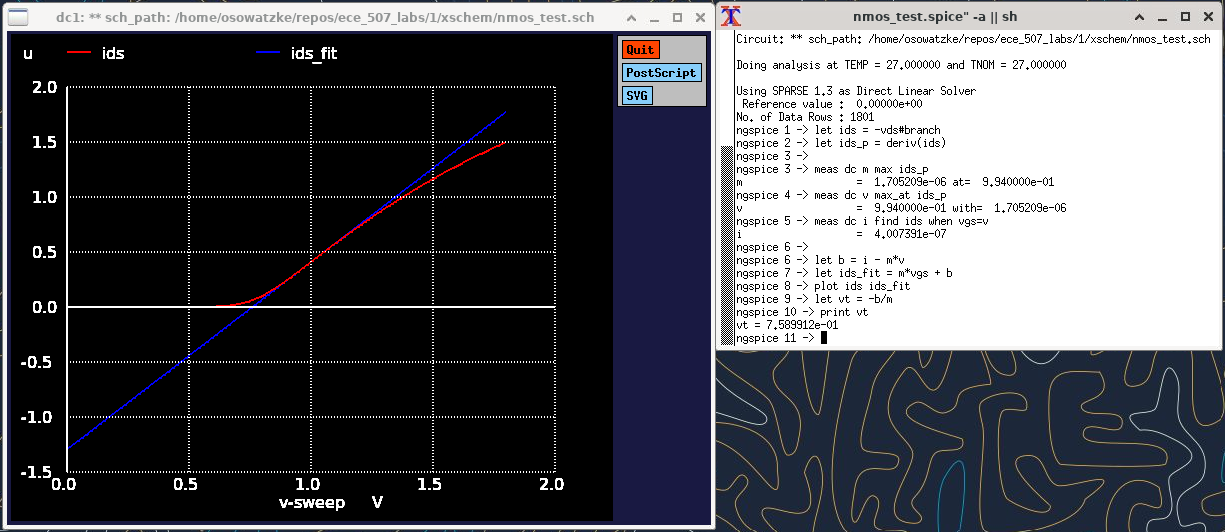
\includegraphics[width=0.8\textwidth]{nmos_vt_meas.png}}
		\caption{Estimating NMOS Threshold Voltage}
		\label{fig::nmos_vt_meas}
	\end{figure}
	
	Next, we measure the saturation voltage. We use the flowchart shown in Figure \ref{fig::nmos_vt_meas_schem} to perform this measurement.
	
	\begin{figure}[H]
		\centerline{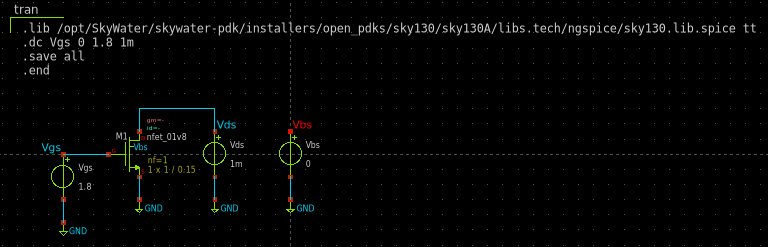
\includegraphics[width=0.8\textwidth]{nmos_vt_meas_schem.png}}
		\caption{NGSPICE Schematic Used to Measure the NMOS Saturation Voltage}
		\label{fig::nmos_vdsat_meas_schem}
	\end{figure}
	
	 \noindent In the above schematic, we consider the drain current in the velocity saturation region. The drain current in this region is defined as follows:
	
	\begin{equation}
		\label{eq::nmos_sat_current}
		I_{ds} = k_n\frac{W_n}{L}\left(V_{gs} - V_{t_n} - \frac{V_{DSAT_n}}{2}\right)V_{DSAT_n}(1 + {\lambda}V_{ds})
	\end{equation}
	
	\noindent If we analyze the ratio of drain currents for the same values of $V_{ds}$ and different values of $V_{gs}$, we can express the ratios as follows:
	
	\begin{equation}
		\frac{V_{gs_1} - V_{t_n} - V_{DSAT_n}/2}{V_{gs_2} - V_{t_n} - V_{DSAT_n}/2} = \frac{V_{gs_1} - V}{V_{gs_2} - V} = \frac{I_{ds_1}}{I_{ds_2}} = \alpha
	\end{equation}
	
	\noindent Solving for $V$, we obtain the following:
	
	\begin{equation}
		V = \frac{{\alpha}V_{gs_2} - V_{gs_1}}{\alpha - 1}
	\end{equation}
	
	\noindent where $V_{DSAT_n} = 2(V - V_{t_n})$. Following the procedure outlined above, we execute the following commands in ngspice to derive the saturation voltage. Our work is shown in Figure \ref{fig::nmos_vt_meas_schem} and we find that $V_{DSAT_n} = 0.202\ \text{V}$.
	
	\begin{figure}[H]
		\centerline{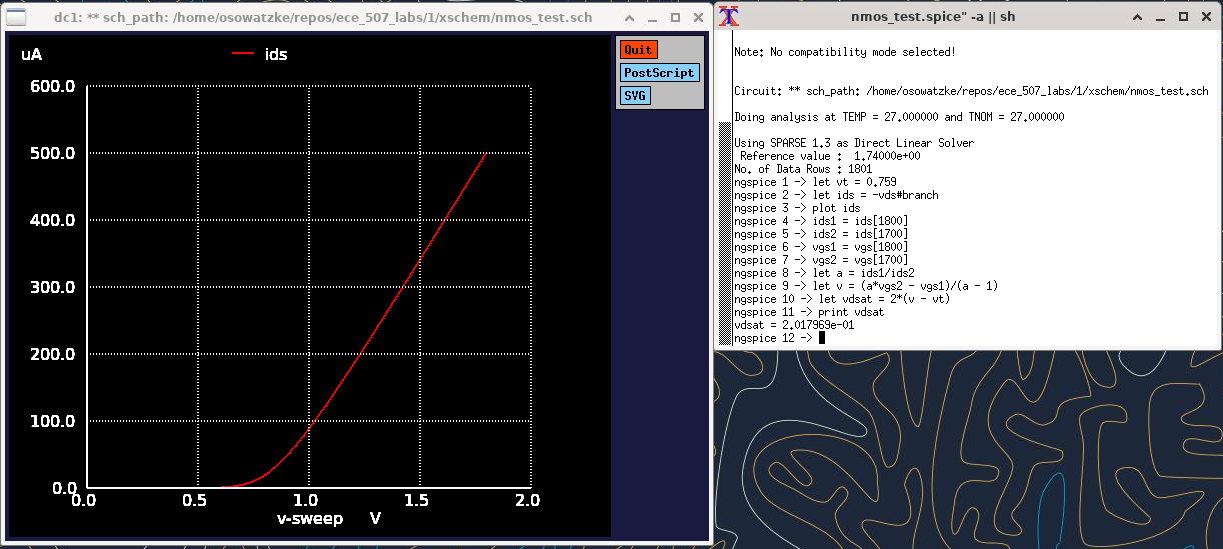
\includegraphics[width=0.8\textwidth]{nmos_vdsat_meas.png}}
		\caption{Measuring the NMOS Saturation Voltage}
		\label{fig::nmos_vdsat_meas}
	\end{figure}
	
	Then, we find the channel length modulation coefficient $\lambda$. To do this, we use the NGSPICE schematic shown in Figure \ref{fig::nmos_lambda_meas_schem}.
	
	\begin{figure}[H]
		\centerline{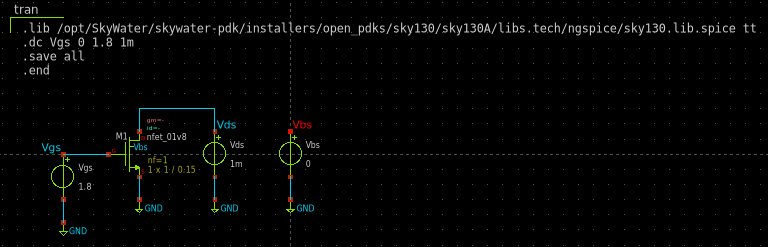
\includegraphics[width=0.8\textwidth]{nmos_vt_meas_schem.png}}
		\caption{NGSPICE Schematic Used to Measure the NMOS Channel Length Modulation Coefficient}
		\label{fig::nmos_lambda_meas_schem}
	\end{figure}
	
	\noindent Here, we once again consider currents in the velocity saturation state. We specifically look at the ratios of currents when varying $V_{ds}$ and keeping $V_{gs}$ constant. Doing so, we obtain the following:
	
	\begin{equation}
		\frac{1 + {\lambda}V_{ds_1}}{1 + {\lambda}V_{ds_2}} = \frac{I_{ds_1}}{I_{ds_2}} = \alpha
	\end{equation}
	
	\noindent Solving for $\lambda$, we obtain the following:
	
	\begin{equation}
		\lambda = \frac{\alpha - 1}{V_{ds_1} - V_{ds_2}}
	\end{equation}
	
	\noindent In Figure \ref{fig::nmos_lambda_meas}, we perform this analysis for the NMOS circuit and find that $\lambda = 0.128 V^{-1}$.
	
	\begin{figure}[H]
		\centerline{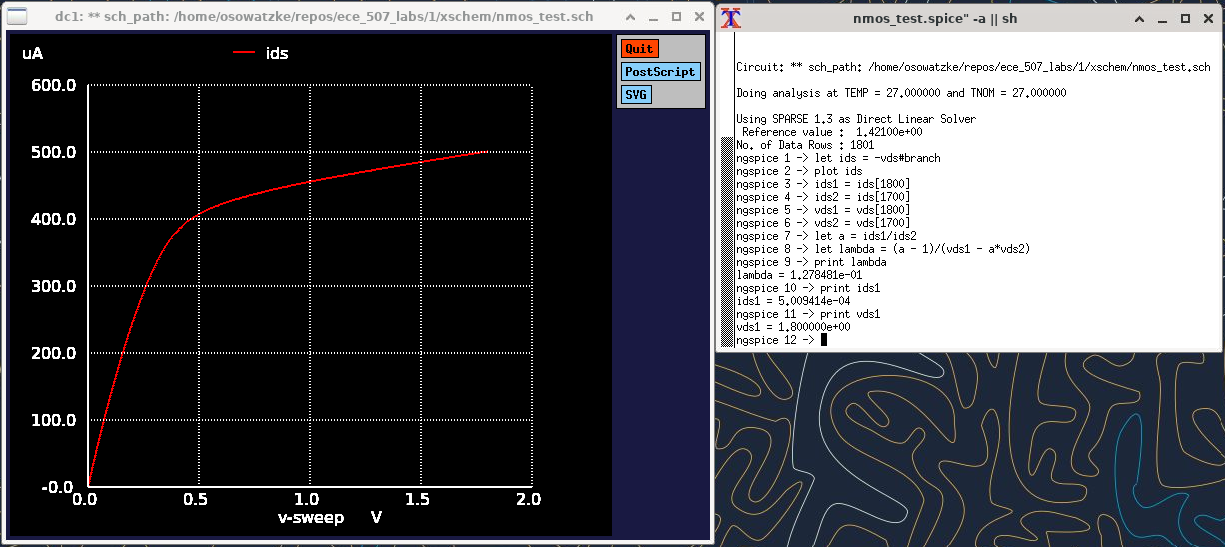
\includegraphics[width=0.8\textwidth]{nmos_lambda_meas.png}}
		\caption{NGSPICE Schematic Used to Measure the NMOS Channel Length Modulation Coefficient}
		\label{fig::nmos_lambda_meas}
	\end{figure}
	
	\noindent Using $\lambda$, we can solve for $k_n$. To do so, we use the current at $V_{ds}=1.8\ \text{V}$ and Equation \ref{eq::nmos_sat_current}. Solving for $k_n$, we obtain:
	
	\begin{equation}
		k_n = I_{ds}\left[\frac{W_n}{L}\left(V_{gs} - V_{t_n} - \frac{V_{DSAT_n}}{2}\right)V_{DSAT_n}(1 + {\lambda}V_{ds})\right]^{-1} = 321.6 {\mu}A/V^2
	\end{equation}
	
	Finally, we can solve for the body effect coefficient, $\gamma$. To do so, we compute the threshold voltage with a non-zero source-to-body voltage, $V_{SB}$. Our test circuit for this measurement is shown in Figure \ref{fig::nmos_gamma_meas_schem}.
	
	 \begin{figure}[H]
		\centerline{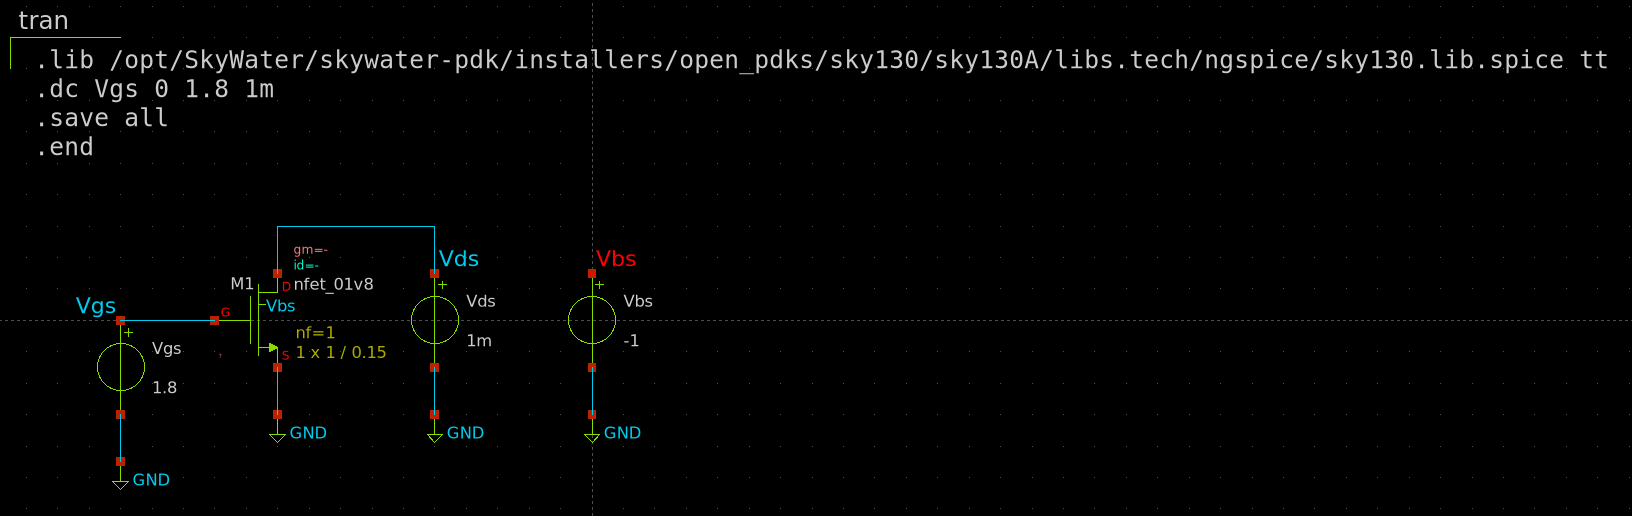
\includegraphics[width=0.8\textwidth]{nmos_gamma_meas_schem.png}}
		\caption{NGSPICE Schematic Used to Measure the NMOS Body Effect Coefficient}
		\label{fig::nmos_gamma_meas_schem}
	\end{figure}
	
	\noindent Using the test circuit, we can measure an updated threshold voltage as follows:
	
	\begin{figure}[H]
		\centerline{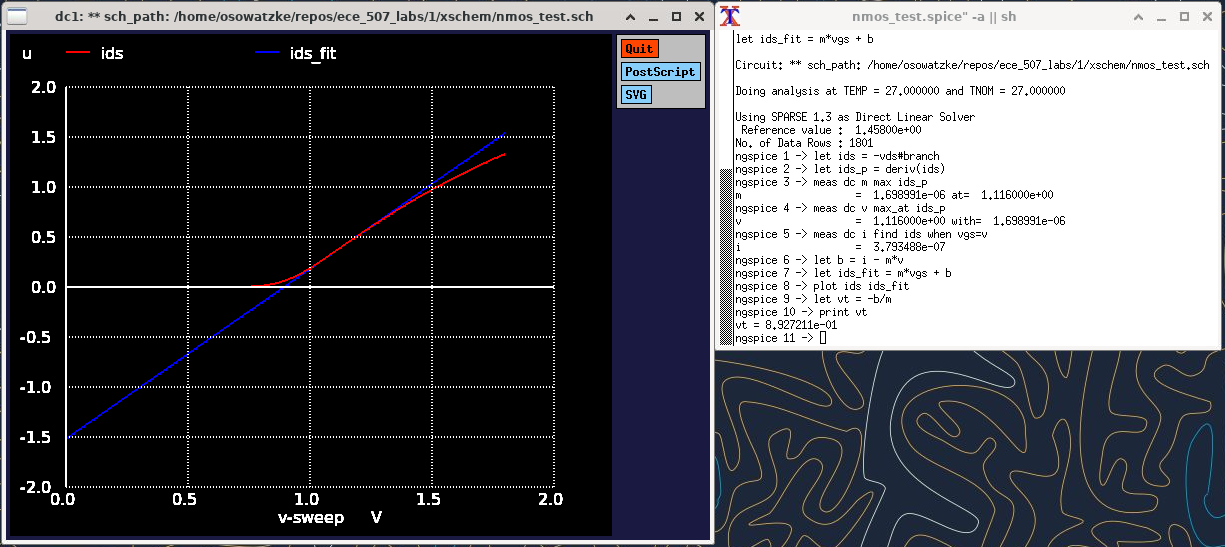
\includegraphics[width=0.8\textwidth]{nmos_gamma_meas.png}}
		\caption{Determine Updated NMOS Threshold Voltage}
		\label{fig::nmos_gamma_meas}
	\end{figure}
	
	\noindent Examining our measured data, we find that $V_T = 0.893 text{V}$. Next, we can solve for the body effect coefficient as follows:
	
	\begin{equation}
		\gamma = \frac{V_T - V_{T_0}}{\sqrt{|-2\phi_F + V_{SB}|} - {\sqrt{|-2\phi_F|}}} 
	\end{equation}
	
	\noindent Assuming $2\phi = -0.6 V$, we find that $\gamma = 0.273 V^{1/2}$. We summarize our results in Table \ref{table::nmos_derived_params}.
	
	\begin{table}[H]
	\begin{center}
	\caption{Derived Parameters for NMOS Gate}
	\label{table::nmos_derived_params}
	\begin{tabular}{| c | c |}
		\hline
		\texttt{Parameter} & \texttt{Value}\\
		\hline	
		$V_{T_0}$ & $0.759\ \text{V}$ \\
		\hline	
		$V_{DSAT}$ & $0.202\ \text{V}$ \\
		\hline	
		$\lambda$ & $0.128\ \text{V}^{-1}$\\
		\hline	
		$k_n$ & $321.6\ {\mu}A/V^2$\\
		\hline	
		$\gamma$ & $0.273\ \text{V}^{1/2}$\\
		\hline
	\end{tabular}
	\end{center}
	\end{table}
	
	\pagebreak
	\section{PMOS IV Characteristics}
	\label{appendix::pmos_iv_characteristics}
	
	In this appendix, we fit a first-order mosfet model to PMOS IV characteristics measured with the sky130A PDK. This enables us to use the equations presented in class to perform first-order analysis of our CMOS gate. We start by estimating the threshold voltage of the PMOS transistor. To perform this measurement, we use the linear extrapolation (or maximum gm) method given in \cite{cmos_vlsi_design}. Our ngspice flowchart for this analysis is given in Figure \ref{fig::pmos_vt_meas_schem}.
	
	\begin{figure}[H]
		\centerline{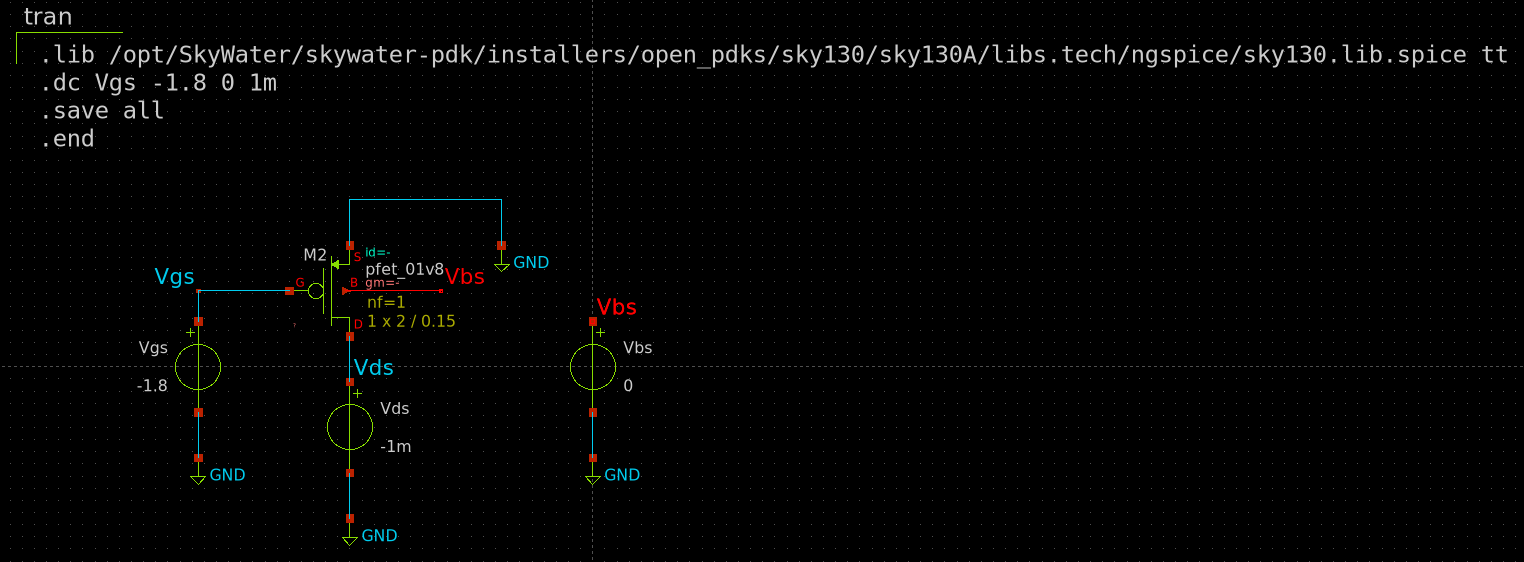
\includegraphics[width=0.8\textwidth]{pmos_vt_meas_schem.png}}
		\caption{NGSPICE Schematic Used to Measure the PMOS Threshold Voltage}
		\label{fig::pmos_vt_meas_schem}
	\end{figure}
	
	\noindent Using the flowchart, we examine the drain current for the PMOS transistor in the linear region of operation. In this region, the drain current of the PMOS transistor is given as follows:
	
	\begin{equation}
		I_{ds} = k_p\frac{W_p}{L}\left(V_{gs} - V_{t_p} - \frac{V_{ds}}{2}\right)V_{ds}
	\end{equation}
	
	\noindent To fit the IV characteristics, we estimate the $I_{ds}$ curve with a line that is tangent to the point with maximum-slope. We then define $V_t$ as the voltage at which the estimated current is zero. This procedure is illustrated in Figure \ref{fig::pmos_vt_meas}, which predicts a threshold voltage of -0.793 V.
	
	\begin{figure}[H]
		\centerline{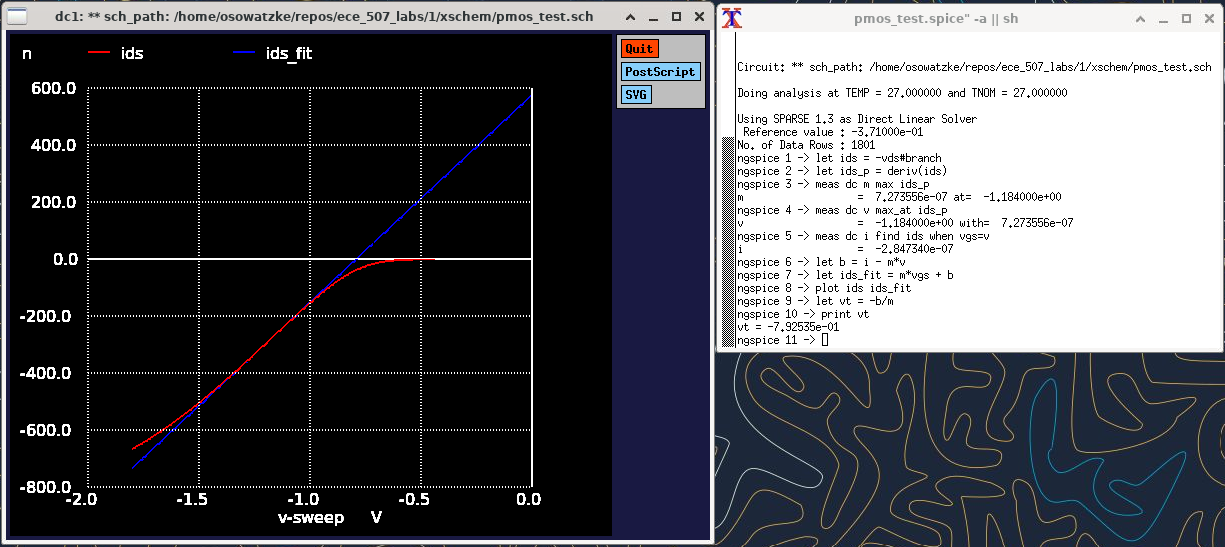
\includegraphics[width=0.8\textwidth]{pmos_vt_meas.png}}
		\caption{Estimating PMOS Threshold Voltage}
		\label{fig::pmos_vt_meas}
	\end{figure}
	
	Next, we measure the saturation voltage. We use the flowchart shown in Figure \ref{fig::pmos_vt_meas_schem} to perform this measurement.
	
	\begin{figure}[H]
		\centerline{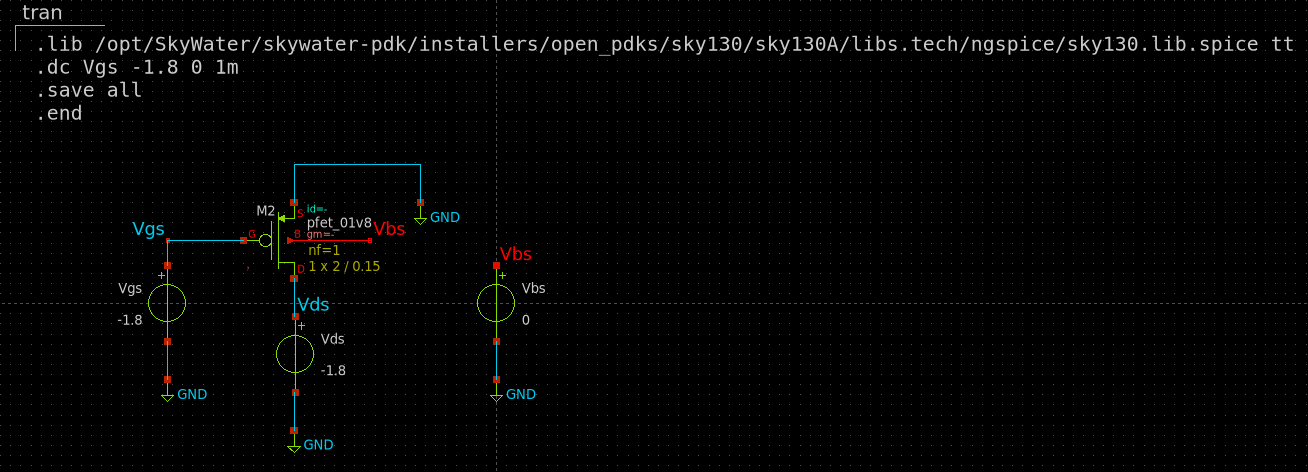
\includegraphics[width=0.8\textwidth]{pmos_vdsat_meas_schem.png}}
		\caption{NGSPICE Schematic Used to Measure the PMOS Saturation Voltage}
		\label{fig::pmos_vdsat_meas_schem}
	\end{figure}
	
	 \noindent In the above schematic, we consider the drain current in the velocity saturation region. The drain current in this region is defined as follows:
	
	\begin{equation}
		\label{eq::pmos_sat_current}
		I_{ds} = k_p\frac{W_p}{L}\left(V_{gs} - V_{t_p} - \frac{V_{DSAT_p}}{2}\right)V_{DSAT_p}(1 + {\lambda}V_{ds})
	\end{equation}
	
	\noindent If we analyze the ratio of drain currents for the same values of $V_{ds}$ and different values of $V_{gs}$, we can express the ratios as follows:
	
	\begin{equation}
		\frac{V_{gs_1} - V_{t_n} - V_{DSAT_p}/2}{V_{gs_2} - V_{t_n} - V_{DSAT_p}/2} = \frac{V_{gs_1} - V}{V_{gs_2} - V} = \frac{I_{ds_1}}{I_{ds_2}} = \alpha
	\end{equation}
	
	\noindent Solving for $V$, we obtain the following:
	
	\begin{equation}
		V = \frac{{\alpha}V_{gs_2} - V_{gs_1}}{\alpha - 1}
	\end{equation}
	
	\noindent where $V_{DSAT_p} = 2(V - V_{t_p})$. Following the procedure outlined above, we execute the following commands in ngspice to derive the saturation voltage. Our work is shown in Figure \ref{fig::pmos_vdsat_meas} and we find that $V_{DSAT_p} = -0.361\ \text{V}$.
	
	\begin{figure}[H]
		\centerline{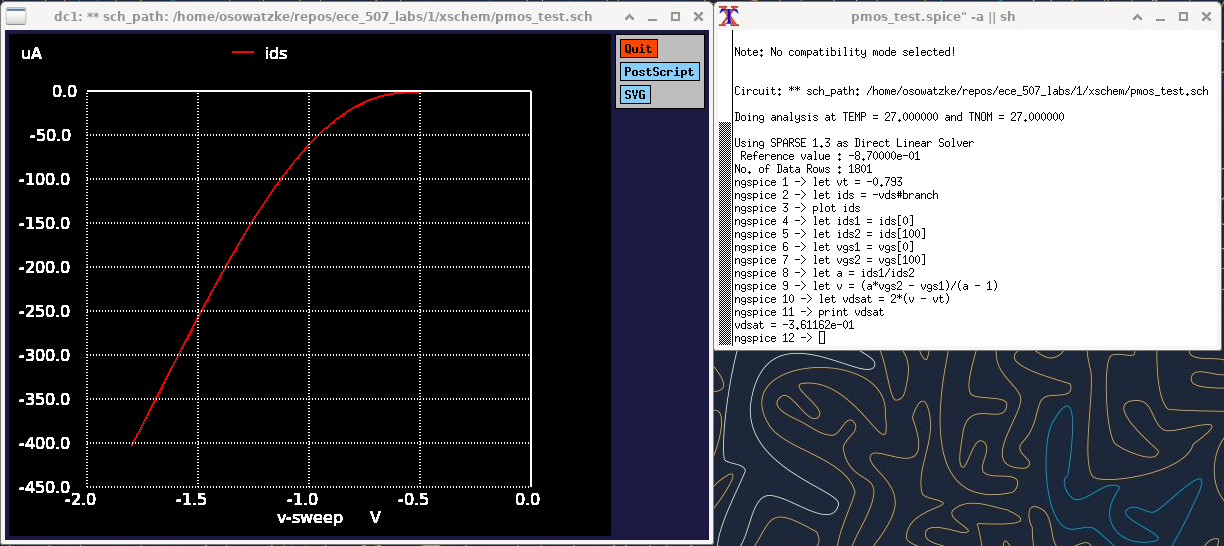
\includegraphics[width=0.8\textwidth]{pmos_vdsat_meas.png}}
		\caption{Measuring the PMOS Saturation Voltage}
		\label{fig::pmos_vdsat_meas}
	\end{figure}
	
	Then, we find the channel length modulation coefficient $\lambda$. To do this, we use the NGSPICE schematic shown in Figure \ref{fig::pmos_lambda_meas_schem}.
	
	\begin{figure}[H]
		\centerline{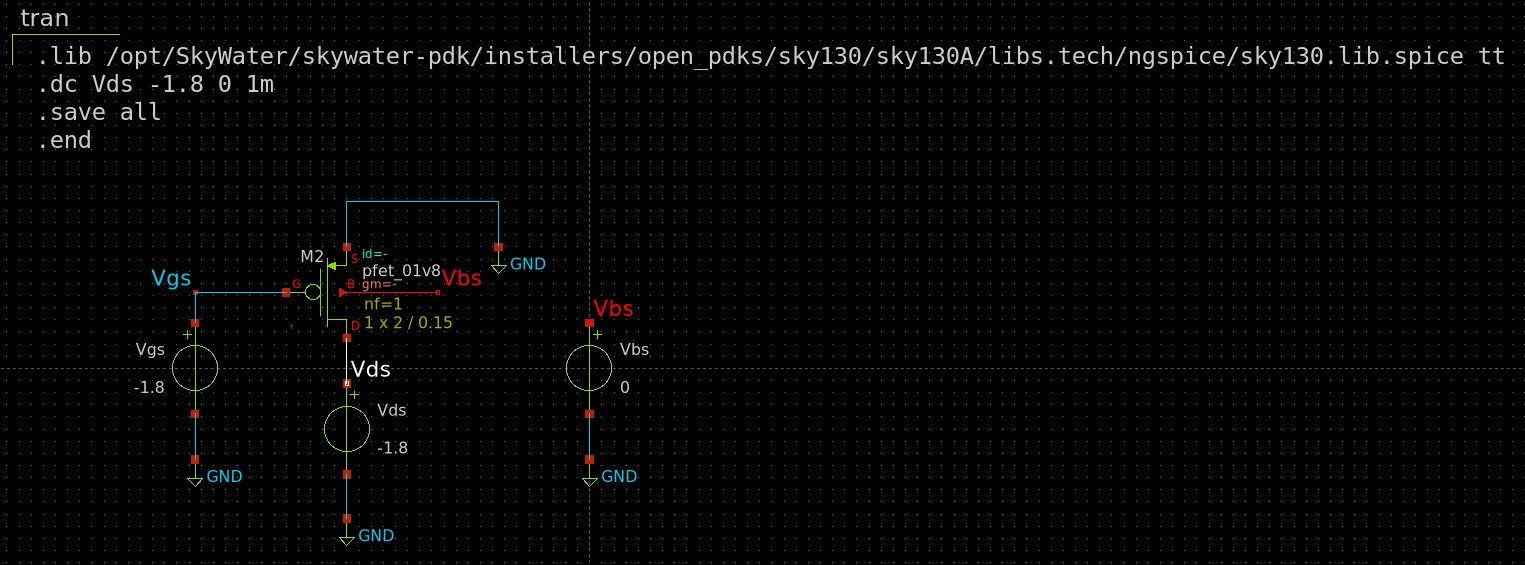
\includegraphics[width=0.8\textwidth]{pmos_lambda_meas_schem.png}}
		\caption{NGSPICE Schematic Used to Measure the PMOS Channel Length Modulation Coefficient}
		\label{fig::pmos_lambda_meas_schem}
	\end{figure}
	
	\noindent Here, we once again consider currents in the velocity saturation state. We specifically look at the ratios of currents when varying $V_{ds}$ and keeping $V_{gs}$ constant. Doing so, we obtain the following:
	
	\begin{equation}
		\frac{1 + {\lambda}V_{ds_1}}{1 + {\lambda}V_{ds_2}} = \frac{I_{ds_1}}{I_{ds_2}} = \alpha
	\end{equation}
	
	\noindent Solving for $\lambda$, we obtain the following:
	
	\begin{equation}
		\lambda = \frac{\alpha - 1}{V_{ds_1} - V_{ds_2}}
	\end{equation}
	
	\noindent In Figure \ref{fig::pmos_lambda_meas}, we perform this analysis for the PMOS circuit and find that $\lambda = -0.335 V^{-1}$.
	
	\begin{figure}[H]
		\centerline{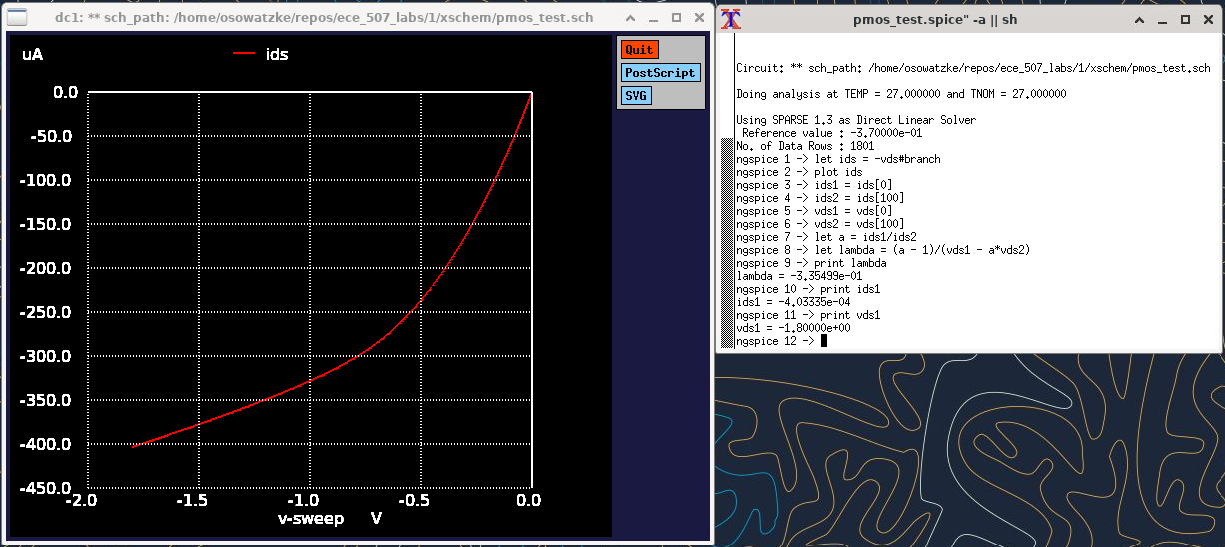
\includegraphics[width=0.8\textwidth]{pmos_lambda_meas.png}}
		\caption{NGSPICE Schematic Used to Measure the PMOS Channel Length Modulation Coefficient}
		\label{fig::pmos_lambda_meas}
	\end{figure}
	
	\noindent Using $\lambda$, we can solve for $k_p$. To do so, we use the current at $V_{ds}=-1.8\ \text{V}$ and Equation \ref{eq::pmos_sat_current}. Solving for $k_p$, we obtain:
	
	\begin{equation}
		k_p = I_{ds}\left[\frac{W_p}{L}\left(V_{gs} - V_{t_p} - \frac{V_{DSAT_p}}{2}\right)V_{DSAT_p}(1 + {\lambda}V_{ds})\right]^{-1} = -63.25 {\mu}A/V^2
	\end{equation}
	
	Finally, we can solve for the body effect coefficient, $\gamma$. To do so, we compute the threshold voltage with a non-zero source-to-body voltage, $V_{SB}$. Our test circuit for this measurement is shown in Figure \ref{fig::pmos_gamma_meas_schem}.
	
	 \begin{figure}[H]
		\centerline{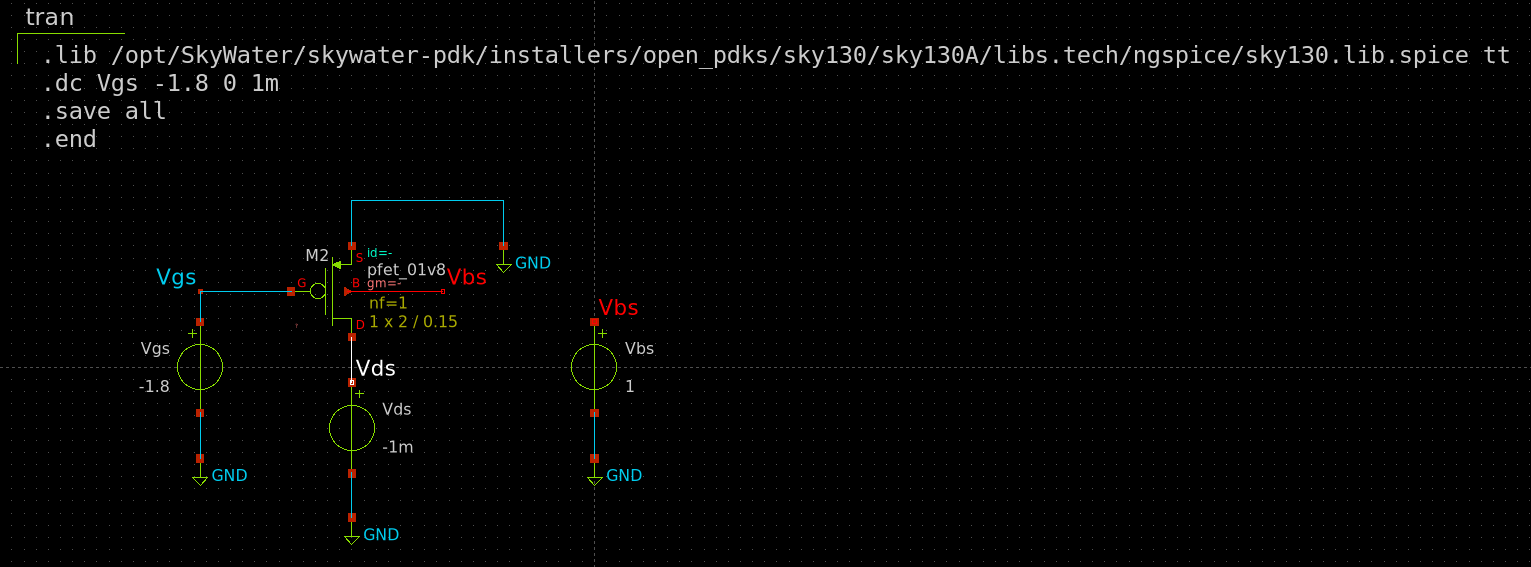
\includegraphics[width=0.8\textwidth]{pmos_gamma_meas_schem.png}}
		\caption{NGSPICE Schematic Used to Measure the PMOS Body Effect Coefficient}
		\label{fig::pmos_gamma_meas_schem}
	\end{figure}
	
	\noindent Using the test circuit, we can measure an updated threshold voltage as follows:
	
	\begin{figure}[H]
		\centerline{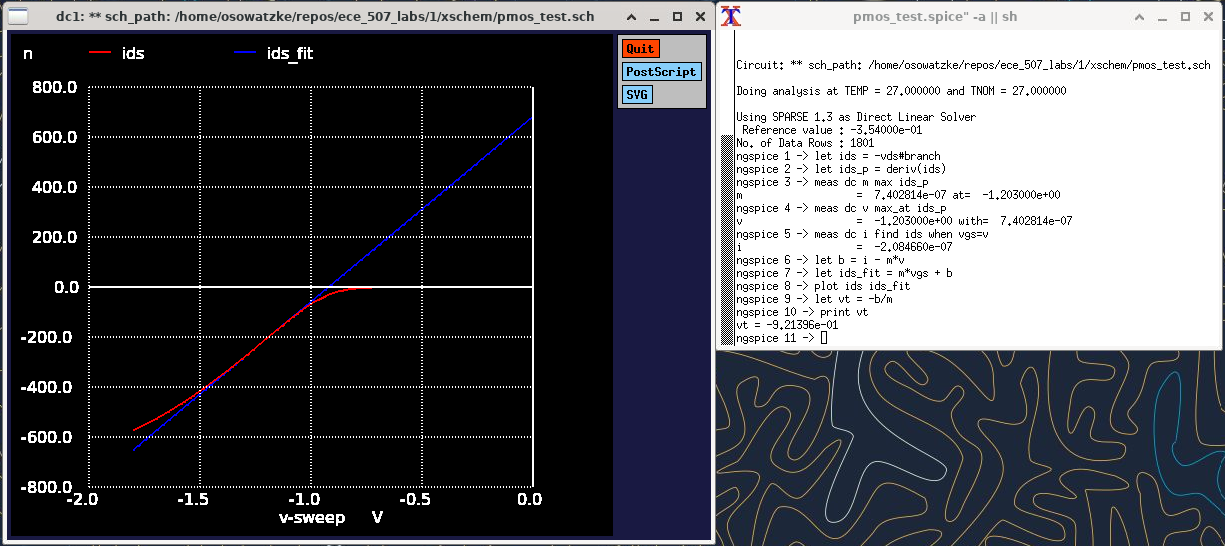
\includegraphics[width=0.8\textwidth]{pmos_gamma_meas.png}}
		\caption{Determine Updated PMOS Threshold Voltage}
		\label{fig::pmos_gamma_meas}
	\end{figure}
	
	\noindent Examining our measured data, we find that $V_T = -0.921\ \text{V}$. Next, we can solve for the body effect coefficient as follows:
	
	\begin{equation}
		\gamma = \frac{V_T - V_{T_0}}{\sqrt{|-2\phi_F - V_{SB}|} - {\sqrt{|-2\phi_F|}}} 
	\end{equation}
	
	\noindent Assuming $2\phi = -0.6 V$, we find that $\gamma = -0.261 V^{1/2}$. We summarize our results in Table \ref{table::pmos_derived_params}.
	
	\begin{table}[H]
	\begin{center}
	\caption{Derived Parameters for PMOS Gate}
	\label{table::pmos_derived_params}
	\begin{tabular}{| c | c |}
		\hline
		\texttt{Parameter} & \texttt{Value}\\
		\hline	
		$V_{T_0}$ & $-0.793\ \text{V}$ \\
		\hline	
		$V_{DSAT}$ & $-0.361\ \text{V}$ \\
		\hline	
		$\lambda$ & $-0.335\ \text{V}^{-1}$\\
		\hline	
		$k_p$ & $-63.25\ {\mu}A/V^2$\\
		\hline	
		$\gamma$ & $-0.261\ \text{V}^{1/2}$\\
		\hline
	\end{tabular}
	\end{center}
	\end{table}
\end{document}